%%=============================================================================
%% LaTeX sjabloon voor bachelorproef, HoGent Bedrijf en Organisatie
%% Opleiding Toegepaste Informatica
%%=============================================================================

\documentclass[fleqn,a4paper,12pt]{book}

%%=============================================================================
%% LaTeX sjabloon voor de bachelorproef, HoGent Bedrijf en Organisatie
%% Opleiding toegepaste informatica
%%
%% Structuur en algemene vormgeving. Meestal hoef je hier niets te wijzigen.
%%
%% Vormgeving gebaseerd op "The Legrand Orange Book", version 2.0 (9/2/15)
%% door Mathias Legrand (legrand.mathias@gmail.com) met aanpassingen door
%% Vel (vel@latextemplates.com). Het oorspronkelijke template is te vinden op
%% http://www.LaTeXTemplates.com
%%
%% Aanpassingen voor HoGent toegepaste informatica: 
%%   Bert Van Vreckem <bert.vanvreckem@hogent.be>
%% Licentie: 
%%   CC BY-NC-SA 3.0 (http://creativecommons.org/licenses/by-nc-sa/3.0/)
%%=============================================================================

%%-----------------------------------------------------------------------------
%% Packages
%%-----------------------------------------------------------------------------

\usepackage[top=3cm,bottom=3cm,left=3cm,right=3cm,headsep=10pt,a4paper]{geometry} % Page margins
\usepackage[utf8]{inputenc}  % Accenten gebruiken in tekst (vb. é ipv \'e)
\usepackage{amsfonts}        % AMS math packages: extra wiskundige
\usepackage{amsmath}         %   symbolen (o.a. getallen-
\usepackage{amssymb}         %   verzamelingen N, R, Z, Q, etc.)
\usepackage[english,dutch]{babel}    % Taalinstellingen: woordsplitsingen,
                             %  commando's voor speciale karakters
                             %  ("dutch" voor NL)
\usepackage{iflang}
\usepackage{eurosym}         % Euro-symbool €
\usepackage{geometry}
\usepackage{graphicx}        % Invoegen van tekeningen
\graphicspath{{img/}}       % Specifies the directory where pictures are stored
\usepackage{tikz}            % Required for drawing custom shapes
\usepackage[pdftex,bookmarks=true]{hyperref}
                             % PDF krijgt klikbare links & verwijzingen,
                             %  inhoudstafel
\usepackage{enumitem}        % Customize lists
\setlist{nolistsep}         % Reduce spacing between list items
\usepackage{listings}        % Broncode mooi opmaken
\usepackage{multirow}        % Tekst over verschillende cellen in tabellen
\usepackage{rotating}        % Tabellen en figuren roteren

\usepackage{booktabs}        % Required for nicer horizontal rules in tables

\usepackage{xcolor}          % Required for specifying colors by name
\definecolor{maincolor}{RGB}{0,147,208} % Define the main color used for 
                             % highlighting throughout the book
                             % 0, 147, 208 = officiële kleur HoGent FBO

% Paragraph style: no indent, add space between paragraphs
\setlength{\parindent}{0em}
\setlength{\parskip}{1em}

\usepackage{etoolbox}
\usepackage{titling} % Macros for title, author, etc
\usepackage{lipsum}          % Voor vultekst (lorem ipsum)

%----------------------------------------------------------------------------------------
%	FONTS
%----------------------------------------------------------------------------------------

\usepackage{avant} % Use the Avantgarde font for headings
%\usepackage{times} % Use the Times font for headings
\usepackage{mathptmx} % Use the Adobe Times Roman as the default text font together with math symbols from the Sym­bol, Chancery and Com­puter Modern fonts

\usepackage{microtype} % Slightly tweak font spacing for aesthetics
\usepackage[utf8]{inputenc} % Required for including letters with accents
\usepackage[T1]{fontenc} % Use 8-bit encoding that has 256 glyphs

%------------------------------------------------------------------------------
%	TITLE PAGE
%------------------------------------------------------------------------------

\newcommand{\inserttitlepage}{%
\begin{titlepage}
  \newgeometry{top=2cm,bottom=1.5cm,left=1.5cm,right=1.5cm}
  \begin{center}

    \begingroup
    \rmfamily
    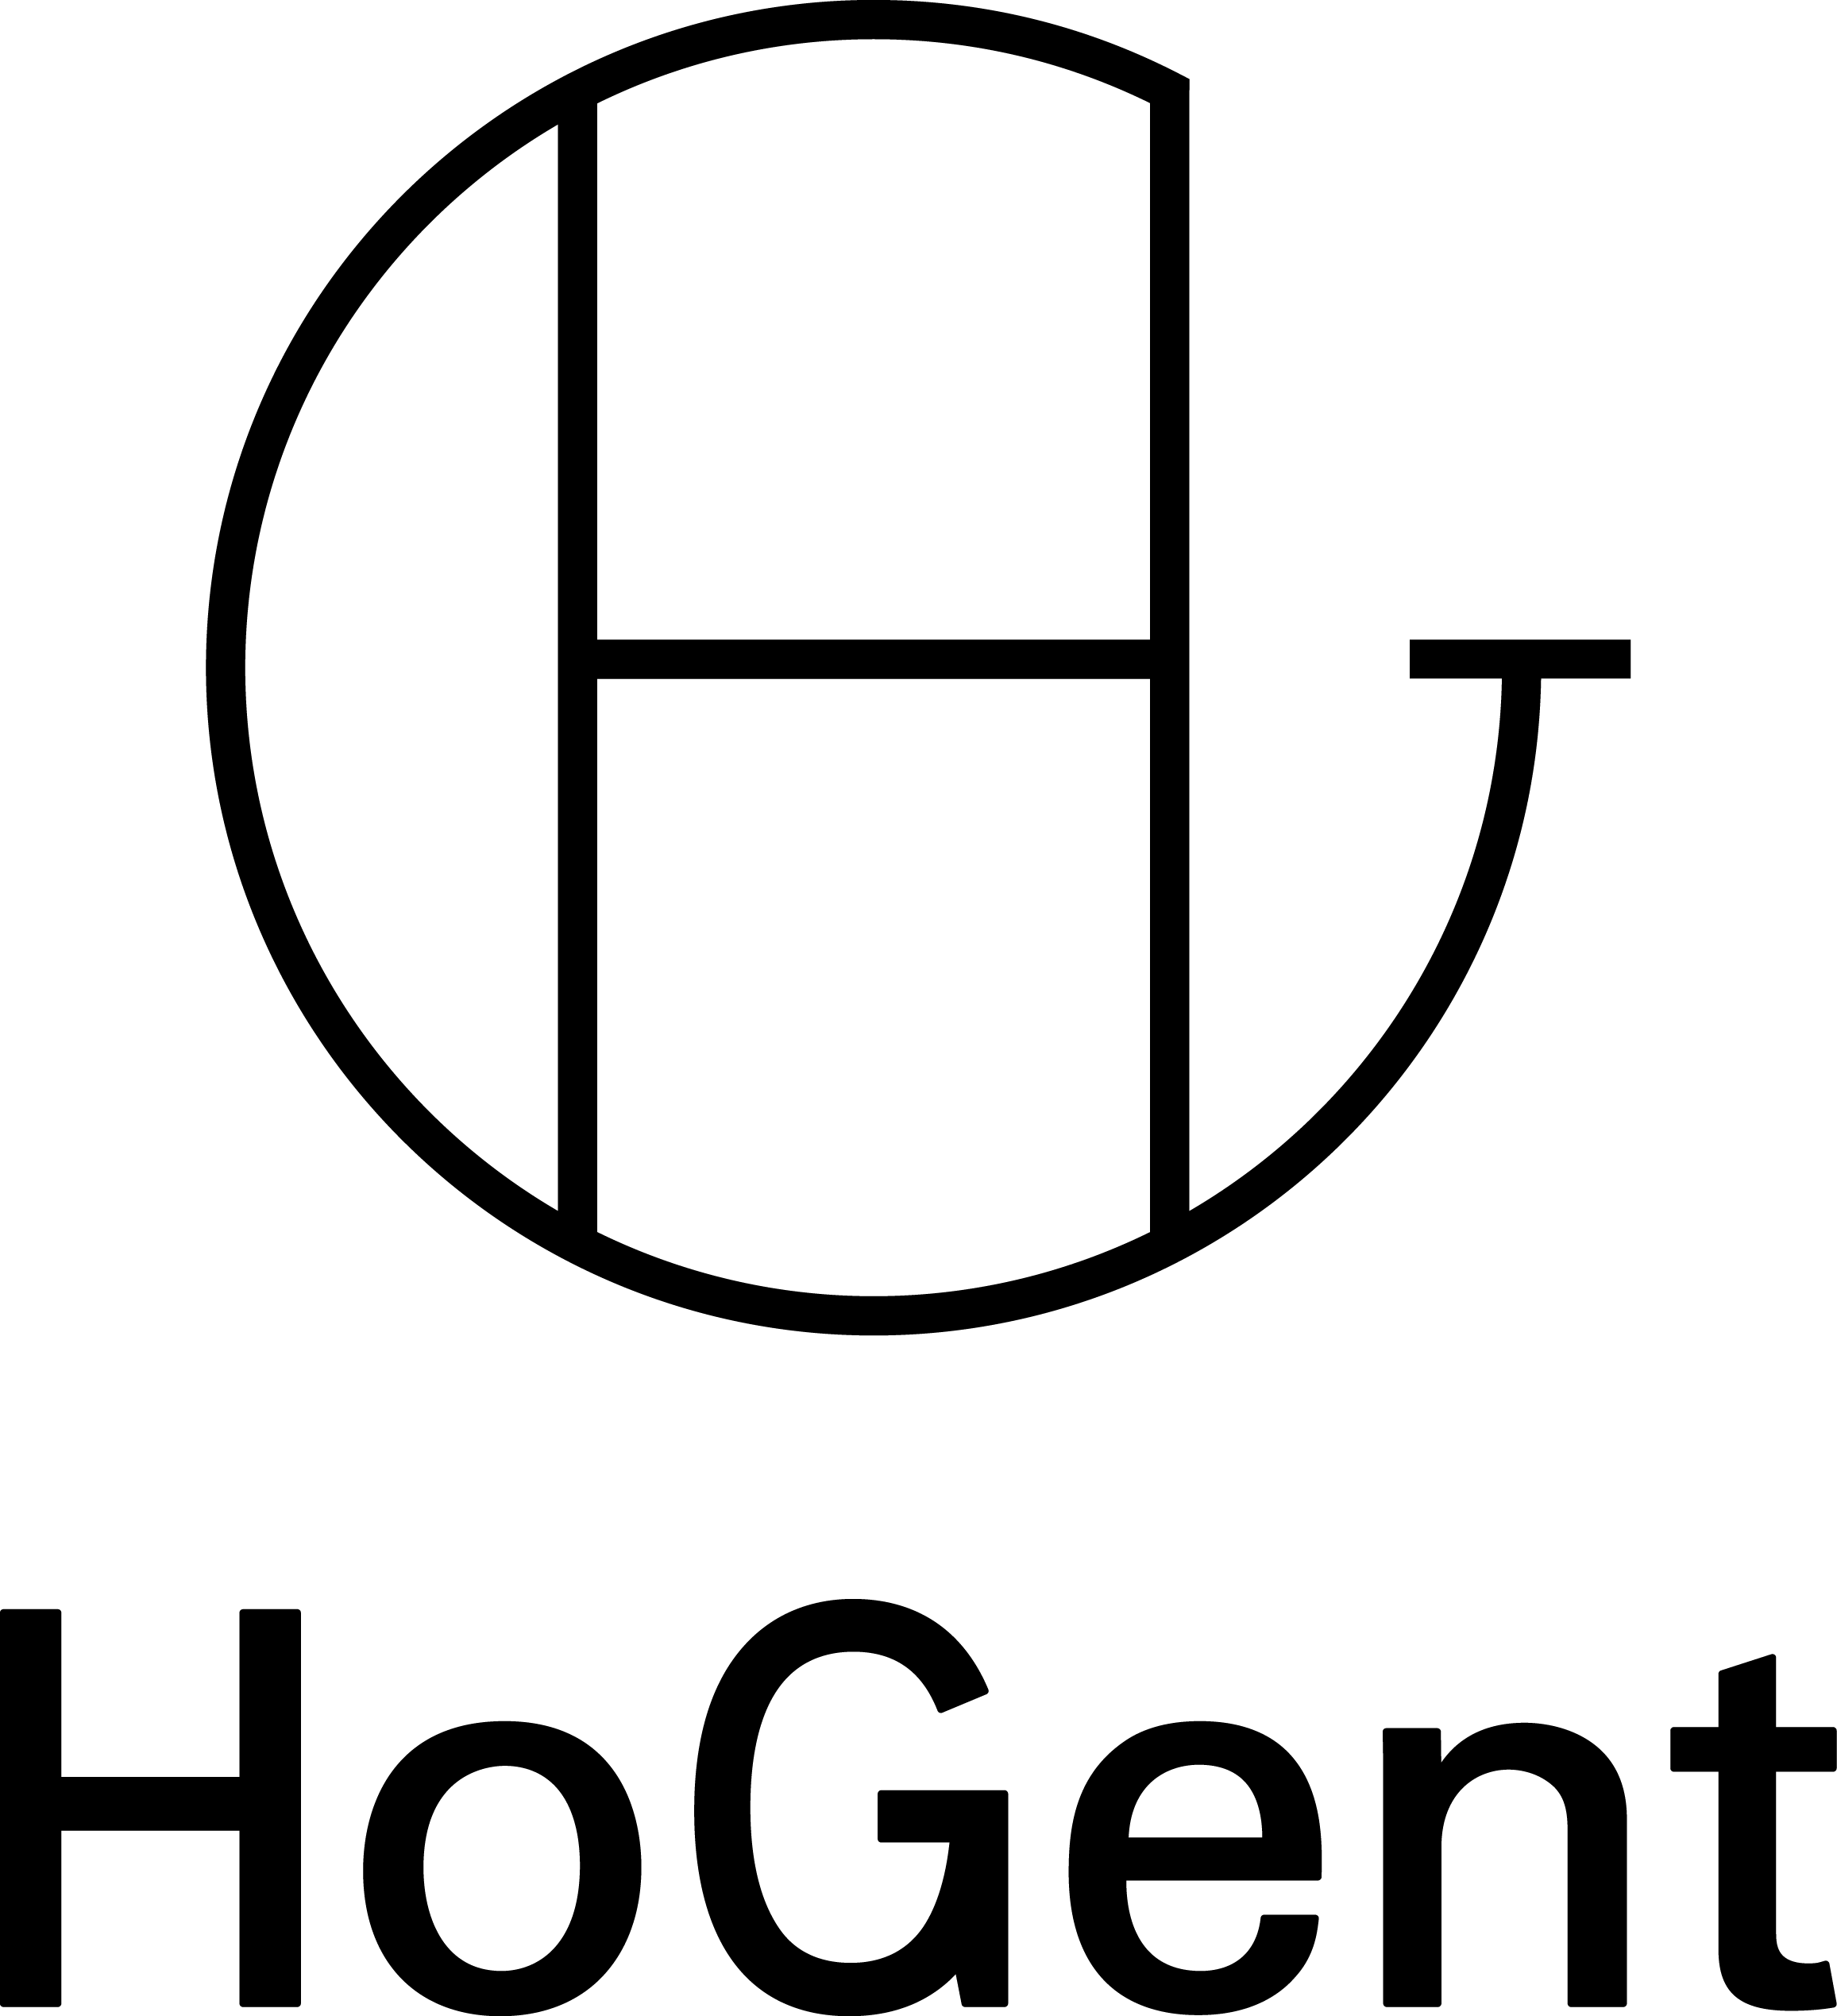
\includegraphics[width=2.5cm]{img/HG-beeldmerk-woordmerk}\\[.5cm]
    Faculteit Bedrijf en Organisatie\\[3cm]
    \titel
    \vfill
    \student\\[3.5cm]
    Scriptie voorgedragen tot het bekomen van de graad van\\professionele bachelor in de toegepaste informatica\\[2cm]
    Promotor:\\
    \promotor\\
    \ifdefempty{\copromotor}{\vspace{2.5cm}}{Co-promotor:\\\copromotor\\[2.5cm]}
    Instelling: \instelling\\[.5cm]
    Academiejaar: \academiejaar\\[.5cm]
    \ifcase \examenperiode \or Eerste \or Tweede \else Derde \fi examenperiode
    \endgroup

  \end{center}
  \restoregeometry
\end{titlepage}
  \emptypage
\begin{titlepage}
  \newgeometry{top=5.35cm,bottom=1.5cm,left=1.5cm,right=1.5cm}
  \begin{center}

    \begingroup
    \rmfamily
    \IfLanguageName{dutch}{Faculteit Bedrijf en Organisatie}{Faculty of Business and Information Management}\\[3cm]
    \titel
    \vfill
    \student\\[3.5cm]
    \IfLanguageName{dutch}{Scriptie voorgedragen tot het bekomen van de graad van\\professionele bachelor in de toegepaste informatica}{Thesis submitted in partial fulfillment of the requirements for the degree of\\professional bachelor of applied computer science}\\[2cm]
    Promotor:\\
    \promotor\\
    \ifdefempty{\copromotor}{\vspace{2.5cm}}{Co-promotor:\\\copromotor\\[2.5cm]}
    \IfLanguageName{dutch}{Instelling}{Institution}: \instelling\\[.5cm]
    \IfLanguageName{dutch}{Academiejaar}{Academic year}: \academiejaar\\[.5cm]
    \IfLanguageName{dutch}{%
    \ifcase \examenperiode \or Eerste \or Tweede \else Derde \fi examenperiode}{%
    \ifcase \examenperiode \or First \or Second \else Third \fi examination period}
    \endgroup

  \end{center}
  \restoregeometry
\end{titlepage}
}

%----------------------------------------------------------------------------------------
%	BIBLIOGRAPHY AND INDEX
%----------------------------------------------------------------------------------------

\usepackage[style=apa,backend=biber]{biblatex}
\usepackage{csquotes}
\DeclareLanguageMapping{dutch}{dutch-apa}
\addbibresource{bachproef-tin.bib} % BibTeX bibliography file
\defbibheading{bibempty}{}

\usepackage{calc} % For simpler calculation - used for spacing the index letter headings correctly
\usepackage{makeidx} % Required to make an index
\makeindex % Tells LaTeX to create the files required for indexing

%----------------------------------------------------------------------------------------
%	MAIN TABLE OF CONTENTS
%----------------------------------------------------------------------------------------

\usepackage{titletoc} % Required for manipulating the table of contents

\contentsmargin{0cm} % Removes the default margin

% Part text styling
\titlecontents{part}[0cm]
{\addvspace{20pt}\centering\large\bfseries}
{}
{}
{}

% Chapter text styling
\titlecontents{chapter}[1.25cm] % Indentation
{\addvspace{12pt}\large\sffamily\bfseries} % Spacing and font options for chapters
{\color{maincolor!60}\contentslabel[\Large\thecontentslabel]{1.25cm}\color{maincolor}} % Chapter number
{\color{maincolor}}
{\color{maincolor!60}\normalsize\;\titlerule*[.5pc]{.}\;\thecontentspage} % Page number

% Section text styling
\titlecontents{section}[1.25cm] % Indentation
{\addvspace{3pt}\sffamily\bfseries} % Spacing and font options for sections
{\contentslabel[\thecontentslabel]{1.25cm}} % Section number
{}
{\hfill\color{black}\thecontentspage} % Page number
[]

% Subsection text styling
\titlecontents{subsection}[1.25cm] % Indentation
{\addvspace{1pt}\sffamily\small} % Spacing and font options for subsections
{\contentslabel[\thecontentslabel]{1.25cm}} % Subsection number
{}
{\ \titlerule*[.5pc]{.}\;\thecontentspage} % Page number
[]

% List of figures
\titlecontents{figure}[0em]
{\addvspace{-5pt}\sffamily}
{\thecontentslabel\hspace*{1em}}
{}
{\ \titlerule*[.5pc]{.}\;\thecontentspage}
[]

% List of tables
\titlecontents{table}[0em]
{\addvspace{-5pt}\sffamily}
{\thecontentslabel\hspace*{1em}}
{}
{\ \titlerule*[.5pc]{.}\;\thecontentspage}
[]

%----------------------------------------------------------------------------------------
%	MINI TABLE OF CONTENTS IN PART HEADS
%----------------------------------------------------------------------------------------

% Chapter text styling
\titlecontents{lchapter}[0em] % Indenting
{\addvspace{15pt}\large\sffamily\bfseries} % Spacing and font options for chapters
{\color{maincolor}\contentslabel[\Large\thecontentslabel]{1.25cm}\color{maincolor}} % Chapter number
{}
{\color{maincolor}\normalsize\sffamily\bfseries\;\titlerule*[.5pc]{.}\;\thecontentspage} % Page number

% Section text styling
\titlecontents{lsection}[0em] % Indenting
{\sffamily\small} % Spacing and font options for sections
{\contentslabel[\thecontentslabel]{1.25cm}} % Section number
{}
{}

% Subsection text styling
\titlecontents{lsubsection}[.5em] % Indentation
{\normalfont\footnotesize\sffamily} % Font settings
{}
{}
{}

%----------------------------------------------------------------------------------------
%	PAGE HEADERS
%----------------------------------------------------------------------------------------

\usepackage{fancyhdr} % Required for header and footer configuration

\pagestyle{fancy}
\renewcommand{\chaptermark}[1]{\markboth{\sffamily\normalsize\bfseries\chaptername\ \thechapter.\ #1}{}} % Chapter text font settings
\renewcommand{\sectionmark}[1]{\markright{\sffamily\normalsize\thesection\hspace{5pt}#1}{}} % Section text font settings
\fancyhf{} \fancyhead[LE,RO]{\sffamily\normalsize\thepage} % Font setting for the page number in the header
\fancyhead[LO]{\rightmark} % Print the nearest section name on the left side of odd pages
\fancyhead[RE]{\leftmark} % Print the current chapter name on the right side of even pages
\renewcommand{\headrulewidth}{0.5pt} % Width of the rule under the header
\addtolength{\headheight}{2.5pt} % Increase the spacing around the header slightly
\renewcommand{\footrulewidth}{0pt} % Removes the rule in the footer
\fancypagestyle{plain}{\fancyhead{}\renewcommand{\headrulewidth}{0pt}} % Style for when a plain pagestyle is specified

% Removes the header from odd empty pages at the end of chapters
\makeatletter
\renewcommand{\cleardoublepage}{
\clearpage\ifodd\c@page\else
\hbox{}
\vspace*{\fill}
\thispagestyle{empty}
\newpage
\fi}

%----------------------------------------------------------------------------------------
%	THEOREM STYLES
%----------------------------------------------------------------------------------------

\usepackage{amsmath,amsfonts,amssymb,amsthm} % For math equations, theorems, symbols, etc

\newcommand{\intoo}[2]{\mathopen{]}#1\,;#2\mathclose{[}}
\newcommand{\ud}{\mathop{\mathrm{{}d}}\mathopen{}}
\newcommand{\intff}[2]{\mathopen{[}#1\,;#2\mathclose{]}}
\newtheorem{notation}{Notation}[chapter]

% Boxed/framed environments
\newtheoremstyle{maincolornumbox}% % Theorem style name
{0pt}% Space above
{0pt}% Space below
{\normalfont}% % Body font
{}% Indent amount
{\small\bf\sffamily\color{maincolor}}% % Theorem head font
{\;}% Punctuation after theorem head
{0.25em}% Space after theorem head
{\small\sffamily\color{maincolor}\thmname{#1}\nobreakspace\thmnumber{\@ifnotempty{#1}{}\@upn{#2}}% Theorem text (e.g. Theorem 2.1)
\thmnote{\nobreakspace\the\thm@notefont\sffamily\bfseries\color{black}---\nobreakspace#3.}} % Optional theorem note
\renewcommand{\qedsymbol}{$\blacksquare$}% Optional qed square

\newtheoremstyle{blacknumex}% Theorem style name
{5pt}% Space above
{5pt}% Space below
{\normalfont}% Body font
{} % Indent amount
{\small\bf\sffamily}% Theorem head font
{\;}% Punctuation after theorem head
{0.25em}% Space after theorem head
{\small\sffamily{\tiny\ensuremath{\blacksquare}}\nobreakspace\thmname{#1}\nobreakspace\thmnumber{\@ifnotempty{#1}{}\@upn{#2}}% Theorem text (e.g. Theorem 2.1)
\thmnote{\nobreakspace\the\thm@notefont\sffamily\bfseries---\nobreakspace#3.}}% Optional theorem note

\newtheoremstyle{blacknumbox} % Theorem style name
{0pt}% Space above
{0pt}% Space below
{\normalfont}% Body font
{}% Indent amount
{\small\bf\sffamily}% Theorem head font
{\;}% Punctuation after theorem head
{0.25em}% Space after theorem head
{\small\sffamily\thmname{#1}\nobreakspace\thmnumber{\@ifnotempty{#1}{}\@upn{#2}}% Theorem text (e.g. Theorem 2.1)
\thmnote{\nobreakspace\the\thm@notefont\sffamily\bfseries---\nobreakspace#3.}}% Optional theorem note

% Non-boxed/non-framed environments
\newtheoremstyle{maincolornum}% % Theorem style name
{5pt}% Space above
{5pt}% Space below
{\normalfont}% % Body font
{}% Indent amount
{\small\bf\sffamily\color{maincolor}}% % Theorem head font
{\;}% Punctuation after theorem head
{0.25em}% Space after theorem head
{\small\sffamily\color{maincolor}\thmname{#1}\nobreakspace\thmnumber{\@ifnotempty{#1}{}\@upn{#2}}% Theorem text (e.g. Theorem 2.1)
\thmnote{\nobreakspace\the\thm@notefont\sffamily\bfseries\color{black}---\nobreakspace#3.}} % Optional theorem note
\renewcommand{\qedsymbol}{$\blacksquare$}% Optional qed square
\makeatother

% Defines the theorem text style for each type of theorem to one of the three styles above
\newcounter{dummy}
\numberwithin{dummy}{section}
\theoremstyle{maincolornumbox}
\newtheorem{theoremeT}[dummy]{Theorem}
\newtheorem{problem}{Problem}[chapter]
\newtheorem{exerciseT}{Exercise}[chapter]
\theoremstyle{blacknumex}
\newtheorem{exampleT}{Example}[chapter]
\theoremstyle{blacknumbox}
\newtheorem{vocabulary}{Vocabulary}[chapter]
\newtheorem{definitionT}{Definition}[section]
\newtheorem{corollaryT}[dummy]{Corollary}
\theoremstyle{maincolornum}
\newtheorem{proposition}[dummy]{Proposition}

%----------------------------------------------------------------------------------------
%	DEFINITION OF COLORED BOXES
%----------------------------------------------------------------------------------------

\RequirePackage[framemethod=default]{mdframed} % Required for creating the theorem, definition, exercise and corollary boxes

% Theorem box
\newmdenv[skipabove=7pt,
skipbelow=7pt,
backgroundcolor=black!5,
linecolor=maincolor,
innerleftmargin=5pt,
innerrightmargin=5pt,
innertopmargin=5pt,
leftmargin=0cm,
rightmargin=0cm,
innerbottommargin=5pt]{tBox}

% Exercise box
\newmdenv[skipabove=7pt,
skipbelow=7pt,
rightline=false,
leftline=true,
topline=false,
bottomline=false,
backgroundcolor=maincolor!10,
linecolor=maincolor,
innerleftmargin=5pt,
innerrightmargin=5pt,
innertopmargin=5pt,
innerbottommargin=5pt,
leftmargin=0cm,
rightmargin=0cm,
linewidth=4pt]{eBox}

% Definition box
\newmdenv[skipabove=7pt,
skipbelow=7pt,
rightline=false,
leftline=true,
topline=false,
bottomline=false,
linecolor=maincolor,
innerleftmargin=5pt,
innerrightmargin=5pt,
innertopmargin=0pt,
leftmargin=0cm,
rightmargin=0cm,
linewidth=4pt,
innerbottommargin=0pt]{dBox}

% Corollary box
\newmdenv[skipabove=7pt,
skipbelow=7pt,
rightline=false,
leftline=true,
topline=false,
bottomline=false,
linecolor=gray,
backgroundcolor=black!5,
innerleftmargin=5pt,
innerrightmargin=5pt,
innertopmargin=5pt,
leftmargin=0cm,
rightmargin=0cm,
linewidth=4pt,
innerbottommargin=5pt]{cBox}

% Creates an environment for each type of theorem and assigns it a theorem text style from the "Theorem Styles" section above and a colored box from above
\newenvironment{theorem}{\begin{tBox}\begin{theoremeT}}{\end{theoremeT}\end{tBox}}
\newenvironment{exercise}{\begin{eBox}\begin{exerciseT}}{\hfill{\color{maincolor}\tiny\ensuremath{\blacksquare}}\end{exerciseT}\end{eBox}}
\newenvironment{definition}{\begin{dBox}\begin{definitionT}}{\end{definitionT}\end{dBox}}
\newenvironment{example}{\begin{exampleT}}{\hfill{\tiny\ensuremath{\blacksquare}}\end{exampleT}}
\newenvironment{corollary}{\begin{cBox}\begin{corollaryT}}{\end{corollaryT}\end{cBox}}

%----------------------------------------------------------------------------------------
%	REMARK ENVIRONMENT
%----------------------------------------------------------------------------------------

\newenvironment{remark}{\par\vspace{10pt}\small % Vertical white space above the remark and smaller font size
\begin{list}{}{
\leftmargin=35pt % Indentation on the left
\rightmargin=25pt}\item\ignorespaces % Indentation on the right
\makebox[-2.5pt]{\begin{tikzpicture}[overlay]
\node[draw=maincolor!60,line width=1pt,circle,fill=maincolor!25,font=\sffamily\bfseries,inner sep=2pt,outer sep=0pt] at (-15pt,0pt){\textcolor{maincolor}{R}};\end{tikzpicture}} % Orange R in a circle
\advance\baselineskip -1pt}{\end{list}\vskip5pt} % Tighter line spacing and white space after remark

%----------------------------------------------------------------------------------------
%	SECTION NUMBERING IN THE MARGIN
%----------------------------------------------------------------------------------------

\makeatletter
\renewcommand{\@seccntformat}[1]{\llap{\textcolor{maincolor}{\csname the#1\endcsname}\hspace{1em}}}
\renewcommand{\section}{\@startsection{section}{1}{\z@}
{-4ex \@plus -1ex \@minus -.4ex}
{1ex \@plus.2ex }
{\normalfont\large\sffamily\bfseries}}
\renewcommand{\subsection}{\@startsection {subsection}{2}{\z@}
{-3ex \@plus -0.1ex \@minus -.4ex}
{0.5ex \@plus.2ex }
{\normalfont\sffamily\bfseries}}
\renewcommand{\subsubsection}{\@startsection {subsubsection}{3}{\z@}
{-2ex \@plus -0.1ex \@minus -.2ex}
{.2ex \@plus.2ex }
{\normalfont\small\sffamily\bfseries}}
\renewcommand\paragraph{\@startsection{paragraph}{4}{\z@}
{-2ex \@plus-.2ex \@minus .2ex}
{.1ex}
{\normalfont\small\sffamily\bfseries}}

%----------------------------------------------------------------------------------------
%	PART HEADINGS
%----------------------------------------------------------------------------------------

% numbered part in the table of contents
\newcommand{\@mypartnumtocformat}[2]{%
\setlength\fboxsep{0pt}%
\noindent\colorbox{maincolor!20}{\strut\parbox[c][.7cm]{\ecart}{\color{maincolor!70}\Large\sffamily\bfseries\centering#1}}\hskip\esp\colorbox{maincolor!40}{\strut\parbox[c][.7cm]{\linewidth-\ecart-\esp}{\Large\sffamily\centering#2}}}%
%%%%%%%%%%%%%%%%%%%%%%%%%%%%%%%%%%
% unnumbered part in the table of contents
\newcommand{\@myparttocformat}[1]{%
\setlength\fboxsep{0pt}%
\noindent\colorbox{maincolor!40}{\strut\parbox[c][.7cm]{\linewidth}{\Large\sffamily\centering#1}}}%
%%%%%%%%%%%%%%%%%%%%%%%%%%%%%%%%%%
\newlength\esp
\setlength\esp{4pt}
\newlength\ecart
\setlength\ecart{1.2cm-\esp}
\newcommand{\thepartimage}{}%
\newcommand{\partimage}[1]{\renewcommand{\thepartimage}{#1}}%
\def\@part[#1]#2{%
\ifnum \c@secnumdepth >-2\relax%
\refstepcounter{part}%
\addcontentsline{toc}{part}{\texorpdfstring{\protect\@mypartnumtocformat{\thepart}{#1}}{\partname~\thepart\ ---\ #1}}
\else%
\addcontentsline{toc}{part}{\texorpdfstring{\protect\@myparttocformat{#1}}{#1}}%
\fi%
\startcontents%
\markboth{}{}%
{\thispagestyle{empty}%
\begin{tikzpicture}[remember picture,overlay]%
\node at (current page.north west){\begin{tikzpicture}[remember picture,overlay]%
\fill[maincolor!20](0cm,0cm) rectangle (\paperwidth,-\paperheight);
\node[anchor=north] at (4cm,-3.25cm){\color{maincolor!40}\fontsize{220}{100}\sffamily\bfseries\@Roman\c@part};
\node[anchor=south east] at (\paperwidth-1cm,-\paperheight+1cm){\parbox[t][][t]{8.5cm}{
\printcontents{l}{0}{\setcounter{tocdepth}{1}}%
}};
\node[anchor=north east] at (\paperwidth-1.5cm,-3.25cm){\parbox[t][][t]{15cm}{\strut\raggedleft\color{white}\fontsize{30}{30}\sffamily\bfseries#2}};
\end{tikzpicture}};
\end{tikzpicture}}%
\@endpart}
\def\@spart#1{%
\startcontents%
\phantomsection
{\thispagestyle{empty}%
\begin{tikzpicture}[remember picture,overlay]%
\node at (current page.north west){\begin{tikzpicture}[remember picture,overlay]%
\fill[maincolor!20](0cm,0cm) rectangle (\paperwidth,-\paperheight);
\node[anchor=north east] at (\paperwidth-1.5cm,-3.25cm){\parbox[t][][t]{15cm}{\strut\raggedleft\color{white}\fontsize{30}{30}\sffamily\bfseries#1}};
\end{tikzpicture}};
\end{tikzpicture}}
\addcontentsline{toc}{part}{\texorpdfstring{%
\setlength\fboxsep{0pt}%
\noindent\protect\colorbox{maincolor!40}{\strut\protect\parbox[c][.7cm]{\linewidth}{\Large\sffamily\protect\centering #1\quad\mbox{}}}}{#1}}%
\@endpart}
\def\@endpart{\vfil\newpage
\if@twoside
\if@openright
\null
\thispagestyle{empty}%
\newpage
\fi
\fi
\if@tempswa
\twocolumn
\fi}

%----------------------------------------------------------------------------------------
%	CHAPTER HEADINGS
%----------------------------------------------------------------------------------------

% A switch to conditionally include a picture, implemented by  Christian Hupfer
\newif\ifusechapterimage
\usechapterimagetrue
\newcommand{\thechapterimage}{}%
\newcommand{\chapterimage}[1]{\ifusechapterimage\renewcommand{\thechapterimage}{#1}\fi}%
\def\@makechapterhead#1{%
{\parindent \z@ \raggedright \normalfont
\ifnum \c@secnumdepth >\m@ne
\if@mainmatter
\begin{tikzpicture}[remember picture,overlay]
\node at (current page.north west)
{\begin{tikzpicture}[remember picture,overlay]
\node[anchor=north west,inner sep=0pt] at (0,0) {\ifusechapterimage\includegraphics[width=\paperwidth]{\thechapterimage}\fi};
\draw[anchor=west] (\Gm@lmargin,-9cm) node [line width=2pt,rounded corners=15pt,draw=maincolor,fill=white,fill opacity=0.5,inner sep=15pt]{\strut\makebox[22cm]{}};
\draw[anchor=west] (\Gm@lmargin+.3cm,-9cm) node {\huge\sffamily\bfseries\color{black}\thechapter. #1\strut};
\end{tikzpicture}};
\end{tikzpicture}
\else
\begin{tikzpicture}[remember picture,overlay]
\node at (current page.north west)
{\begin{tikzpicture}[remember picture,overlay]
\node[anchor=north west,inner sep=0pt] at (0,0) {\ifusechapterimage\includegraphics[width=\paperwidth]{\thechapterimage}\fi};
\draw[anchor=west] (\Gm@lmargin,-9cm) node [line width=2pt,rounded corners=15pt,draw=maincolor,fill=white,fill opacity=0.5,inner sep=15pt]{\strut\makebox[22cm]{}};
\draw[anchor=west] (\Gm@lmargin+.3cm,-9cm) node {\huge\sffamily\bfseries\color{black}#1\strut};
\end{tikzpicture}};
\end{tikzpicture}
\fi\fi\par\vspace*{270\p@}}}

%-------------------------------------------

\def\@makeschapterhead#1{%
\begin{tikzpicture}[remember picture,overlay]
\node at (current page.north west)
{\begin{tikzpicture}[remember picture,overlay]
\node[anchor=north west,inner sep=0pt] at (0,0) {\ifusechapterimage\includegraphics[width=\paperwidth]{\thechapterimage}\fi};
\draw[anchor=west] (\Gm@lmargin,-9cm) node [line width=2pt,rounded corners=15pt,draw=maincolor,fill=white,fill opacity=0.5,inner sep=15pt]{\strut\makebox[22cm]{}};
\draw[anchor=west] (\Gm@lmargin+.3cm,-9cm) node {\huge\sffamily\bfseries\color{black}#1\strut};
\end{tikzpicture}};
\end{tikzpicture}
\par\vspace*{270\p@}}
\makeatother

%----------------------------------------------------------------------------------------
%	HYPERLINKS IN THE DOCUMENTS
%----------------------------------------------------------------------------------------

\usepackage{hyperref}
\hypersetup{hidelinks,backref=true,pagebackref=true,hyperindex=true,colorlinks=false,breaklinks=true,urlcolor= maincolor,bookmarks=true,bookmarksopen=false,pdftitle={Title},pdfauthor={Author}}
\usepackage{bookmark}
\bookmarksetup{
open,
numbered,
addtohook={%
\ifnum\bookmarkget{level}=0 % chapter
\bookmarksetup{bold}%
\fi
\ifnum\bookmarkget{level}=-1 % part
\bookmarksetup{color=maincolor,bold}%
\fi
}
}

%----------------------------------------------------------------------------------------
%	Java source code
%----------------------------------------------------------------------------------------

% Commando voor invoegen Java-broncodebestanden (dank aan Niels Corneille)
% Gebruik:
%   \codefragment{source/MijnKlasse.java}{Uitleg bij de code}
%
% Je kan dit aanpassen aan de taal die je zelf het meeste gebruikt in je
% bachelorproef.
\newcommand{\codefragment}[2]{ \lstset{%
  language=java,
  breaklines=true,
  float=th,
  caption={#2},
  basicstyle=\scriptsize,
  frame=single,
  extendedchars=\true
}
\lstinputlisting{#1}}

% Leeg blad
\newcommand{\emptypage}{%
\newpage
\thispagestyle{empty}
\mbox{}
\newpage
}


%%---------- Documenteigenschappen --------------------------------------------
%% TODO: Vul dit aan met je eigen info:

% Je eigen naam
\newcommand{\student}{Gianni Stubbe}

% De naam van je promotor (lector van de opleiding)
\newcommand{\promotor}{Jens Buysse}

% De naam van je co-promotor. Als je promotor ook je opdrachtgever is en je
% dus ook inhoudelijk begeleidt (en enkel dan!), mag je dit leeg laten.
\newcommand{\copromotor}{Bert Van Vreckem}

% Indien je bachelorproef in opdracht van/in samenwerking met een bedrijf of
% externe organisatie geschreven is, geef je hier de naam. Zoniet laat je dit
% zoals het is.
\newcommand{\instelling}{---}

% De titel van het rapport/bachelorproef
\newcommand{\titel}{Automatische opzet van Cisco IOS netwerkapparatuur in combinatie met Ansible}

% Datum van indienen (gebruik telkens de deadline, ook al geef je eerder af)
\newcommand{\datum}{26 augustus 2016}

% Academiejaar
\newcommand{\academiejaar}{2015-2016}

% Examenperiode
%  - 1e semester = 1e examenperiode => 1
%  - 2e semester = 2e examenperiode => 2
%  - tweede zit  = 3e examenperiode => 3
\newcommand{\examenperiode}{3}

%%=============================================================================
%% Inhoud document
%%=============================================================================

\begin{document}

%---------- Titelblad ---------------------------------------------------------
\inserttitlepage

%---------- Samenvatting, voorwoord -------------------------------------------
\usechapterimagefalse
%%=============================================================================
%% Samenvatting
%%=============================================================================

%% TODO: De "abstract" of samenvatting is een kernachtige (~ 1 blz. voor een
%% thesis) synthese van het document.
%%
%% Deze aspecten moeten zeker aan bod komen:
%% - Context: waarom is dit werk belangrijk?
%% - Nood: waarom moest dit onderzocht worden?
%% - Taak: wat heb je precies gedaan?
%% - Object: wat staat in dit document geschreven?
%% - Resultaat: wat was het resultaat?
%% - Conclusie: wat is/zijn de belangrijkste conclusie(s)?
%% - Perspectief: blijven er nog vragen open die in de toekomst nog kunnen
%%    onderzocht worden? Wat is een mogelijk vervolg voor jouw onderzoek?
%%
%% LET OP! Een samenvatting is GEEN voorwoord!

%%---------- Nederlandse samenvatting -----------------------------------------
%%
%% TODO: Als je je bachelorproef in het Engels schrijft, moet je eerst een
%% Nederlandse samenvatting invoegen. Haal daarvoor onderstaande code uit
%% commentaar.
%% Wie zijn bachelorproef in het Nederlands schrijft, kan dit negeren en heel
%% deze sectie verwijderen.

\IfLanguageName{english}{%
\selectlanguage{dutch}
\chapter*{Samenvatting}
\lipsum[1-4]
\selectlanguage{english}
}{}

%%---------- Samenvatting -----------------------------------------------------
%%
%% De samenvatting in de hoofdtaal van het document

\chapter*{\IfLanguageName{dutch}{Samenvatting}{Abstract}}

\lipsum[1-4]

%%=============================================================================
%% Voorwoord
%%=============================================================================

\chapter*{Voorwoord}
\label{ch:voorwoord}

%% TODO:
%% Het voorwoord is het enige deel van de bachelorproef waar je vanuit je
%% eigen standpunt (``ik-vorm'') mag schrijven. Je kan hier bv. motiveren
%% waarom jij het onderwerp wil bespreken.
%% Vergeet ook niet te bedanken wie je geholpen/gesteund/... heeft

Het onderwerp in kwestie is gekozen geweest door mijn interesse in Ansible op zich. Twee jaar geleden heb ik de eerste hands-on gekregen in de les van Mr. Van Vreckem waar het me al snel aansprak. Nu enkele jaren later blijkt Ansible op veel verschillende plaatsen al gebruikt te worden, dit merk ik ook in het dagelijkse leven. 
\\

Een van de aspecten waar ik hier mee in aanraking kom is binnen 'Frag-O-Matic', dit is een Lanparty in België die gemiddeld een duizendtal bezoekers trekt per editie. Hier merkte ik dat zo goed als alles die zij deden op servers in playbooks gegoten waren voor Ansible. Een van de aspecten waar wel nog veel werk aan is zijn de netwerkswitches en dergelijke. 
\\
Hier viel mij het nieuwe onderwerp in: Ansible met netwerkapparatuur. Na een beetje zoeken merkte ik snel dat dit het geschikte moment was om het onderzoek te verrichten omdat de technologie nog maar sinds kort als eerste stable versie naar buiten werd gebracht. Al snel werd mij terug duidelijk waarom ik Ansible nu ook weer zo tof vond, nu werd dit dan ook nog eens gecombineerd met Cisco apparaten.
\\

Als laatste wil ik Stefanie Geldof en haar broer bedanken voor het gebruik van de Cisco 2960 Series switch, zonder dit was het niet mogelijk geweest dit onderzoek te verrichten. 
Ook BeSports en Frag-O-Matic wil ik bedanken om mij in aanraking te brengen met het idee voor iets dergelijk. Automatisatie voor een Lanparty lijkt me heel handig maar het is door hen dat ik met het idee kwam.
\\

Ik wens de lezer veel leesplezier toe, welkom in de wereld van automatisatie.

%---------- Inhoudstafel ------------------------------------------------------
\pagestyle{empty} % No headers
\tableofcontents % Print the table of contents itself
\cleardoublepage % Forces the first chapter to start on an odd page so it's on the right
\pagestyle{fancy} % Print headers again

%---------- Lijst afkortingen, termen -----------------------------------------
%% Als je een lijst van afkortingen of termen wil toevoegen, dan hoort die
%% hier thuis. Gebruik bijvoorbeeld de ``glossaries'' package.

%%---------- Kern -------------------------------------------------------------

%%=============================================================================
%% Inleiding
%%=============================================================================

\chapter{Inleiding}
\label{ch:inleiding}

De inleiding moet de lezer alle nodige informatie verschaffen om het onderwerp te begrijpen zonder nog externe werken te moeten raadplegen \autocite{Pollefliet2011}. Dit is een doorlopende tekst die gebaseerd is op al wat je over het onderwerp gelezen hebt (literatuuronderzoek).

Je verwijst bij elke bewering die je doet, vakterm die je introduceert, enz. naar je bronnen. In \LaTeX{} kan dat met het commando \texttt{$\backslash${textcite\{\}}} of \texttt{$\backslash${autocite\{\}}}. Als argument van het commando geef je de ``sleutel'' van een ``record'' in een bibliografische databank in het Bib\TeX{}-formaat (een tekstbestand). Als je expliciet naar de auteur verwijst in de zin, gebruik je \texttt{$\backslash${}textcite\{\}}.
Soms wil je de auteur niet expliciet vernoemen, dan gebruik je \texttt{$\backslash${}autocite\{\}}. Hieronder een voorbeeld van elk.

\textcite{Knuth1998} schreef een van de standaardwerken over sorteer- en zoekalgoritmen. Experten zijn het erover eens dat cloud computing een interessante opportuniteit vormen, zowel voor gebruikers als voor dienstverleners op vlak van informatietechnologie~\autocite{Creeger2009}.

\section{Stand van zaken}
\label{sec:stand-van-zaken}

%% TODO: deze sectie (die je kan opsplitsen in verschillende secties) bevat je
%% literatuurstudie. Vergeet niet telkens je bronnen te vermelden!

\lipsum[7-20]

\section{Probleemstelling en Onderzoeksvragen}
\label{sec:onderzoeksvragen}

%% TODO:
%% Uit je probleemstelling moet duidelijk zijn dat je onderzoek een meerwaarde
%% heeft voor een concrete doelgroep (bv. een bedrijf).
%%
%% Wees zo concreet mogelijk bij het formuleren van je
%% onderzoeksvra(a)g(en). Een onderzoeksvraag is trouwens iets waar nog
%% niemand op dit moment een antwoord heeft (voor zover je kan nagaan).

\section{Opzet van deze bachelorproef}
\label{sec:opzet-bachelorproef}

%% TODO: Het is gebruikelijk aan het einde van de inleiding een overzicht te
%% geven van de opbouw van de rest van de tekst. Deze sectie bevat al een aanzet
%% die je kan aanvullen/aanpassen in functie van je eigen tekst.

De rest van deze bachelorproef is als volgt opgebouwd:

In Hoofdstuk~\ref{ch:methodologie} wordt de methodologie toegelicht en worden de gebruikte onderzoekstechnieken besproken om een antwoord te kunnen formuleren op de onderzoeksvragen.

%% TODO: Vul hier aan voor je eigen hoofstukken, één of twee zinnen per hoofdstuk

In Hoofdstuk~\ref{ch:conclusie}, tenslotte, wordt de conclusie gegeven en een antwoord geformuleerd op de onderzoeksvragen. Daarbij wordt ook een aanzet gegeven voor toekomstig onderzoek binnen dit domein.


%%=============================================================================
%% Methodologie
%%=============================================================================

\chapter{Methodologie}
\label{ch:methodologie}

\section{Onderzoek naar mogelijkheden}
\label{ch:mogelijkheden}

Eerst en vooral werd er gezocht naar wat de mogelijkheden zijn de dag van vandaag in vergelijking met een jaar geleden. Omdat dit vooral rond Ansible draait is er dus eerst naar dat onderdeel gekeken. Het is belangrijk dat het onderzoek toekomstgericht is en dus ook met de laatste mogelijkheden werkt. Omdat er heel veel vooruitgang geboekt wordt binnen deze sector is het dus cruciaal dat dit documentatie gebruikt die zo up-to-date mogelijk is. 
\\

Hiervoor werd er gezocht op verschillende fora, er werd gekeken naar de blogposts van Ansible zelf en heel vaak wordt er ook gekeken op Github repositories. Deze zijn vaak een heel goede indicatie van in hoeverre een project nog actief ondersteund wordt en deze nog verder ontwikkeld wordt. Iets die meer dan een jaar geen commit meer heeft ontvangen kan je zo goed als niet nuttig beschouwen in vergelijking met de projecten die de laatste jaar op gang zijn gekomen. 
\\

Heel vaak werd er ook door documentatie gegaan om te kijken wat mogelijk was met welke tools om te zien of dit voldoet aan wat we willen bereiken. Goede documentatie is ook een belangrijke factor om het project goed te kunnen gebruiken in het verdere proces. Ook maakt dit ook heel veel uit om de keuze voor een bepaald pakket eenvoudiger te maken. 

\section{Uitwerking basis configuratie}
\label{ch:configuratie}

Om het configureren op de test te stellen moet er eerst een basis configuratie voor handen zijn. Dit is hoe het eindresultaat zou moeten zijn na het uitvoeren van gelijk welke automatisatie methode. Als dit niet zo is dan kunnen we beslissen dat het gebruik van een bepaalde techniek niet geschikt is voor dagelijks gebruik of implementatie in een bedrijfsinfrastructuur.
\\

De basisconfiguratie zal zich richten op Cisco IOS apparatuur meer bepaald wat voor handen is. Hoofdzakelijk zal er gewerkt worden met een 2960 series switch die voor dit onderzoek ten allen tijde beschikbaar was. De configuratie zal vooral inwerken op enkel basiscommando's die in het dagelijks leven het meest gebruikt worden. Hieronder valt bijvoorbeeld VLAN tagging en bijvoorbeeld ip adressering. 

\section{Automatiseren van configuratie}
\label{ch:automatiseren}

Als laatste hebben we dan nog het belangrijkste aspect van dit onderzoek, dit zijnde het automatiseren van de configuratie die bereikt is met de bovenstaande methode. Er zal gestart worden van een bepaalde basisconfiguratie, dit het liefst zo dicht mogelijk bij een factory reset. Dus er wordt ook gekeken naar hoeveel werk er op voorhand nodig is om alles werkende te kunnen krijgen via een automatisch platform zoals Ansible. Ook moet er rekening gehouden worden met de configuratie in combinatie met Ansible. Hoeverre kan het automatiseren voor problemen zorgen bijvoorbeeld als Ansible een ip adres verandert en zichzelf zo buitensluit bijvoorbeeld. Dit probleem heeft dan ook te maken met dat Ansible voor netwerkapparatuur over SSH loopt die een geldige ip adressering nodig heeft om te kunnen werken.
\\

Net zoals het configureren van een server zal er ook eerst gekeken worden naar de stappen die manueel nodig zijn om het resultaat te behalen. Daarna zullen deze stappen overgezet worden in 'Tasks' zoals dit binnen Ansible noemt. Het voordeel vergeleken met een server role is dat de stappen bij een switch en router veel eenduidiger zullen zijn. Het installeren van een DNS server op Linux is net iets ingewikkelder dan de commando's laten uitvoeren binnen Ansible die nodig zijn om een Cisco apparaat te configureren.



%% TODO: Hoe ben je te werk gegaan? Verdeel je onderzoek in grote fasen, en
%% licht in elke fase toe welke stappen je gevolgd hebt. Verantwoord waarom je
%% op deze manier te werk gegaan bent. Je moet kunnen aantonen dat je de best
%% mogelijke manier toegepast hebt om een antwoord te vinden op de
%% onderzoeksvraag.



%%=============================================================================
%% Methodologie
%%=============================================================================

\chapter{Testopstelling}
\label{ch:testopstelling}
 
Om dit alles te testen werd er gebruik gemaakt van een Cisco 2960 Series switch die geproduceerd is in 2006. Het model van deze is meer bepaald de C2960-24LT die een 24 100Mbit poorten heeft waarvan er acht voorzien zijn van POE. Als laatste zijn er nog twee Gigabit interfaces aanwezig. De switch had versie 12.2(44R)SE1 geïnstalleerd bij het uitvoeren van de tests.
Deze kwam nieuw uit de doos dus stond deze bij het ontvangen volledig op standaardinstellingen. Hierna werd er gekeken hoe we de werkelijkheid zoveel mogelijk konden nabootsen. Daarom is de switch tijdens het configureren over SSH achter een router geplaatst. Op deze manier was het bijvoorbeeld ook heel eenvoudig om via een laptop op afstand en over een WiFi-netwerk het apparaat te beheren, ongeveer zoals dit in werkelijkheid zou verlopen.
\\

Omdat er voor het instellen van de basisconfiguratie nog nood is aan een console connectie werd een seriële kabel met usb aansluiting aangekocht, dit is goedkoop terug te vinden op Ebay en werk met nieuwere computers prettig en hiervoor was ook geen installatie nodig. Dit was noodzakelijk omdat veel computers tegenwoordig geen DB9 aansluiting meer hebben, hoewel dit de enige kabel is die meegeleverd wordt met een Cisco switch.

\begin{figure}[H]
\centering
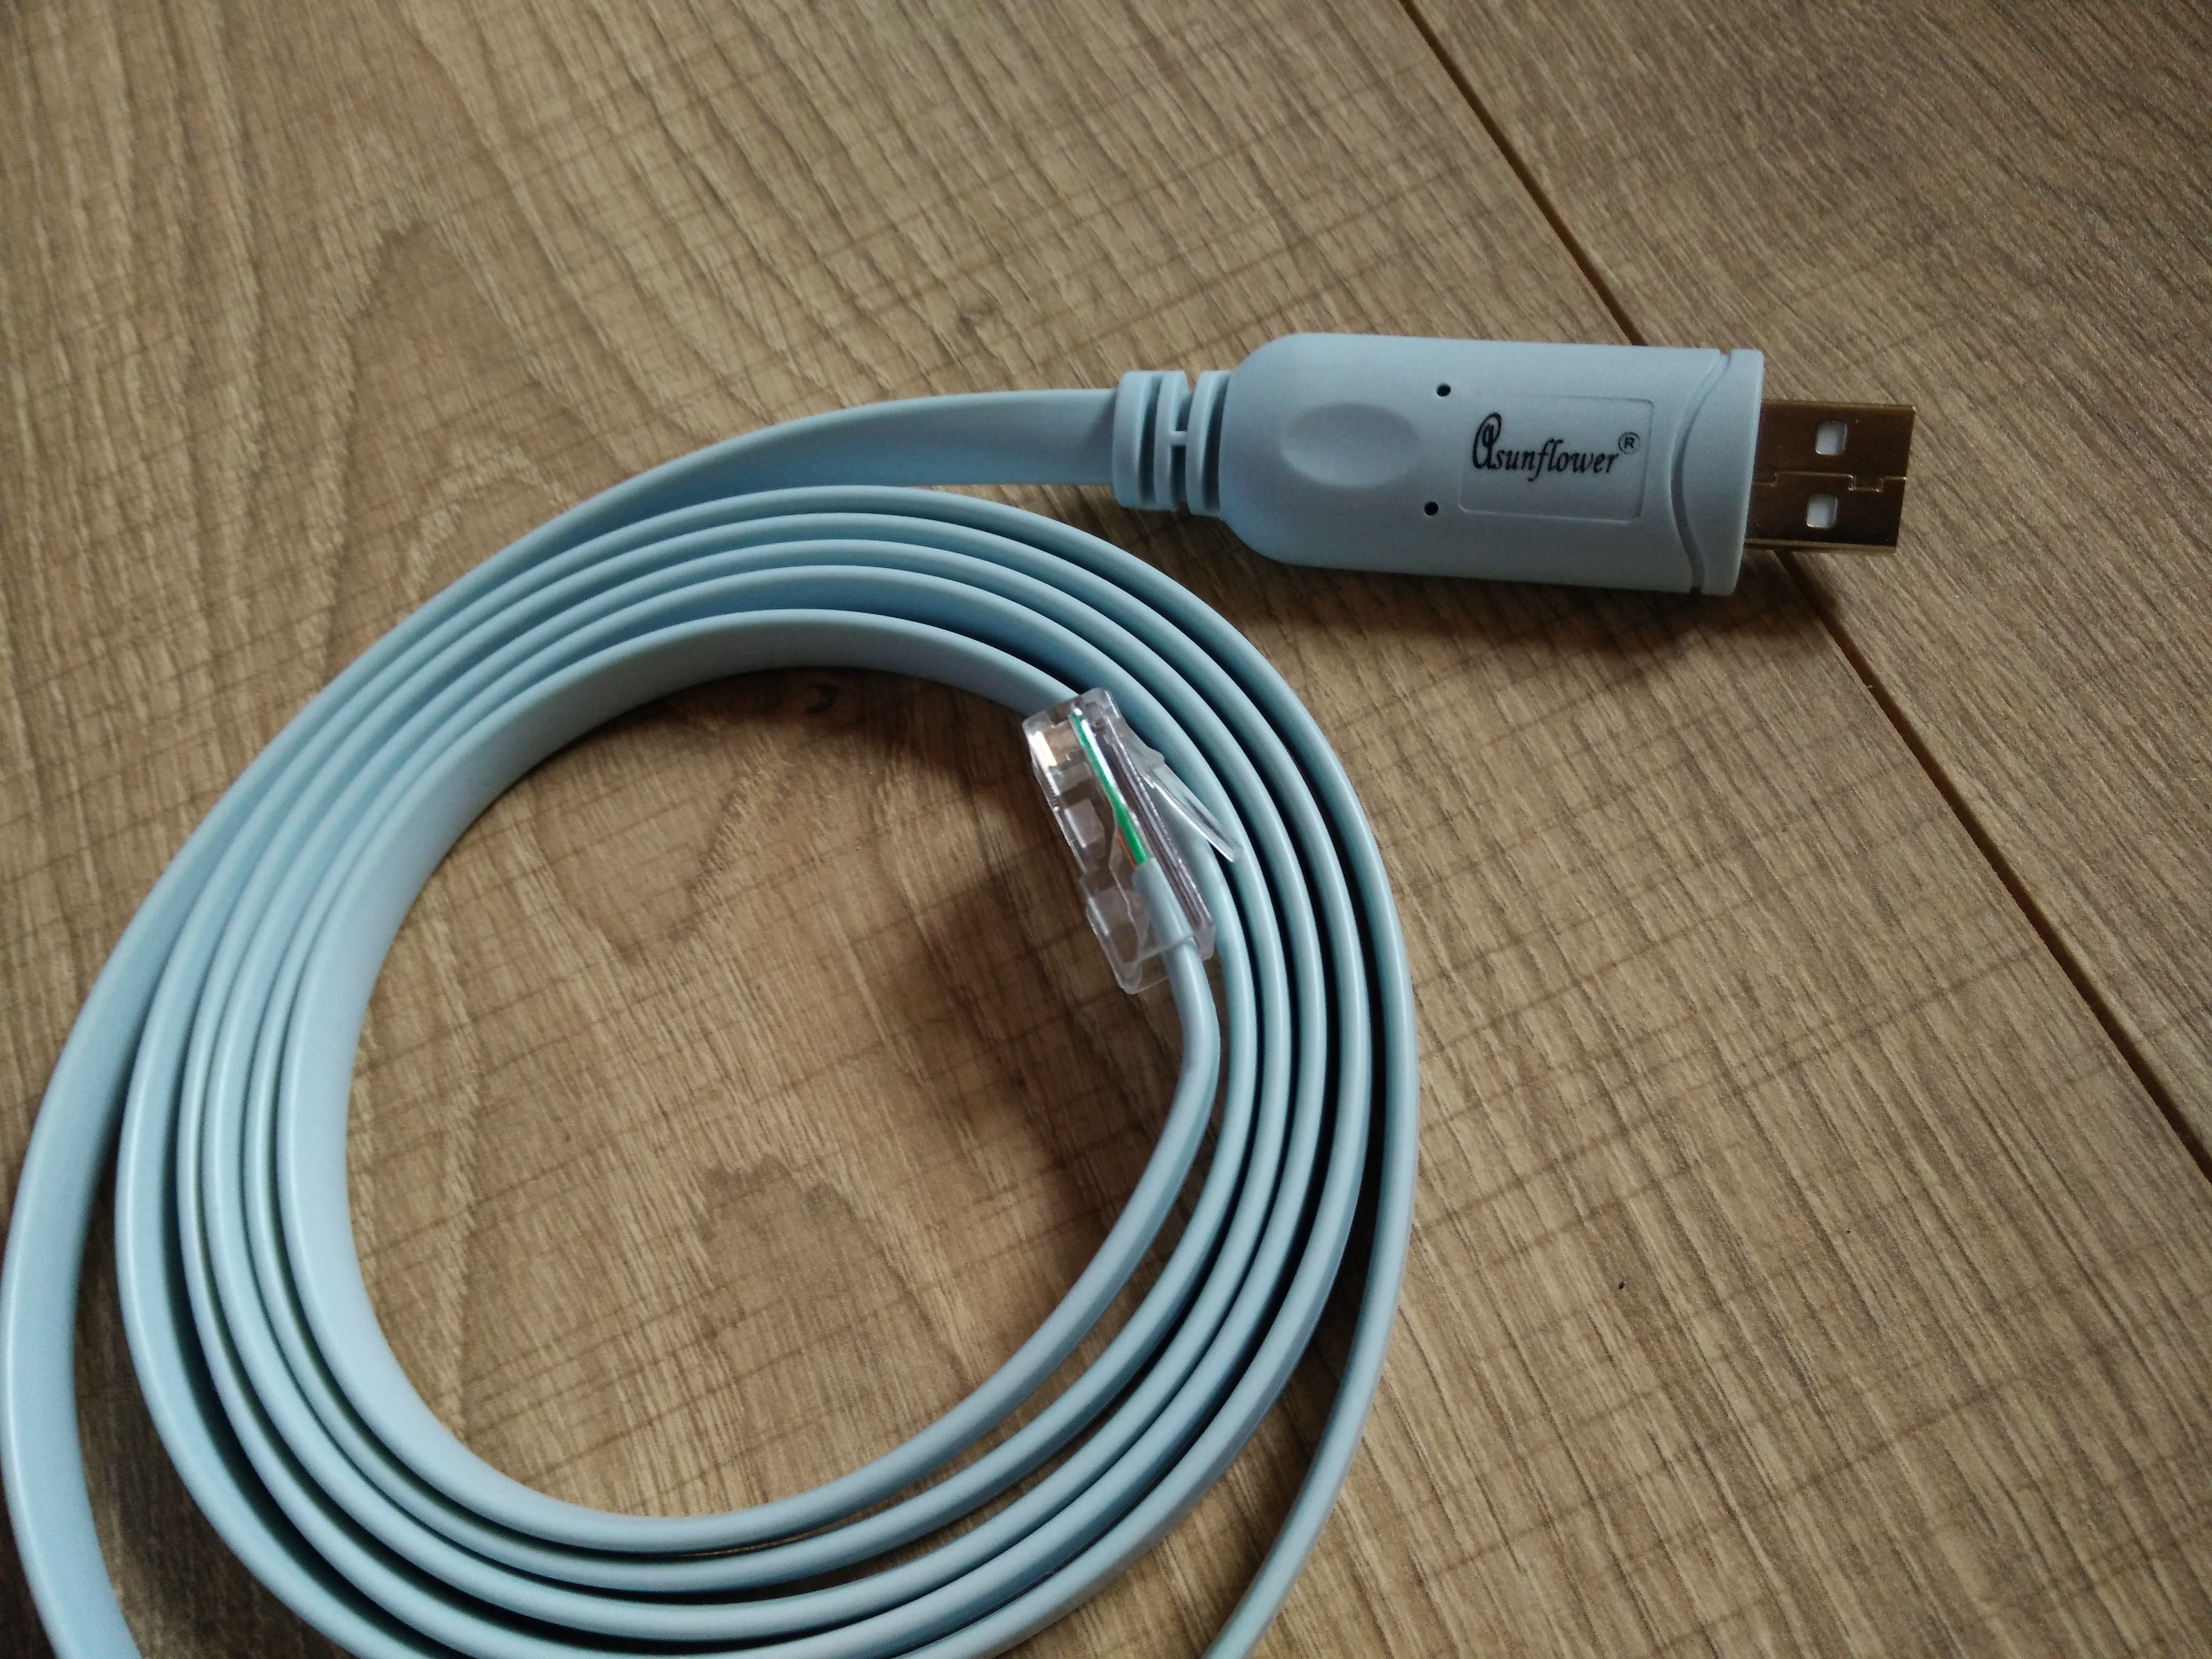
\includegraphics[width=10cm]{../img/serialcable}
\caption{De aangekochte seriële consolekabel, deze is te vinden op Ebay als een 'FTDI USB to RJ45'. Er wordt ook duidelijk vermeld dat dit specifiek voor Cisco apparaten is. }
\end{figure}

Om deze in gebruik te nemen bij Windows is het even kijken onder apparaatbeheer welke poort deze precies in beslag neemt. Dit kan je terug vinden onder de sectie 'poorten'. Op mijn apparaat was dit COM4. Hierna kan je in Putty bij seriële connectie gewoon COM1 aanpassen naar COM4 en de juiste snelheid meegeven, dit staat standaard correct maar indien dit niet zo is moet het 9600 zijn. Daarna kan je aan de slag met het apparaat zoals gewoonlijk.
\\

Op een Apple computer is de procedure een klein beetje anders. Het is een beetje zoeken hoe het apparaat precies noemt maar via tabcompletion is het vrij eenvoudig terug te vinden.
\begin{center}
\begin{BVerbatim}
$ screen /dev/tty.usb
	% invoer van tab
$ screen /dev/tty.usbserial-AK05D1K3
switch1>
\end{BVerbatim}
\end{center}

Verder is het noodzakelijk om op de switch een ip adres in te stellen en een default gateway. Enkel op deze manier is het mogelijk om een connectie vanop afstand te maken met de switch. Verder om een SSH verbinding tot stand te kunnen brengen is er een username en een wachtwoord nodig, ook dit moet ingesteld worden. Als laatste wordt een SSH key aangemaakt. Vanaf dan is het mogelijk om via SSH connectie te maken, zoals je met een server zou doen. Dit kan via Putty op Windows of via het SSH commando op bijna ieder unix systeem. Dit is hoe Ansible en NAPALM connectie zullen maken met het apparaat dus deze stap is cruciaal voor het verdere proces.
\begin{figure}[H]
\centering
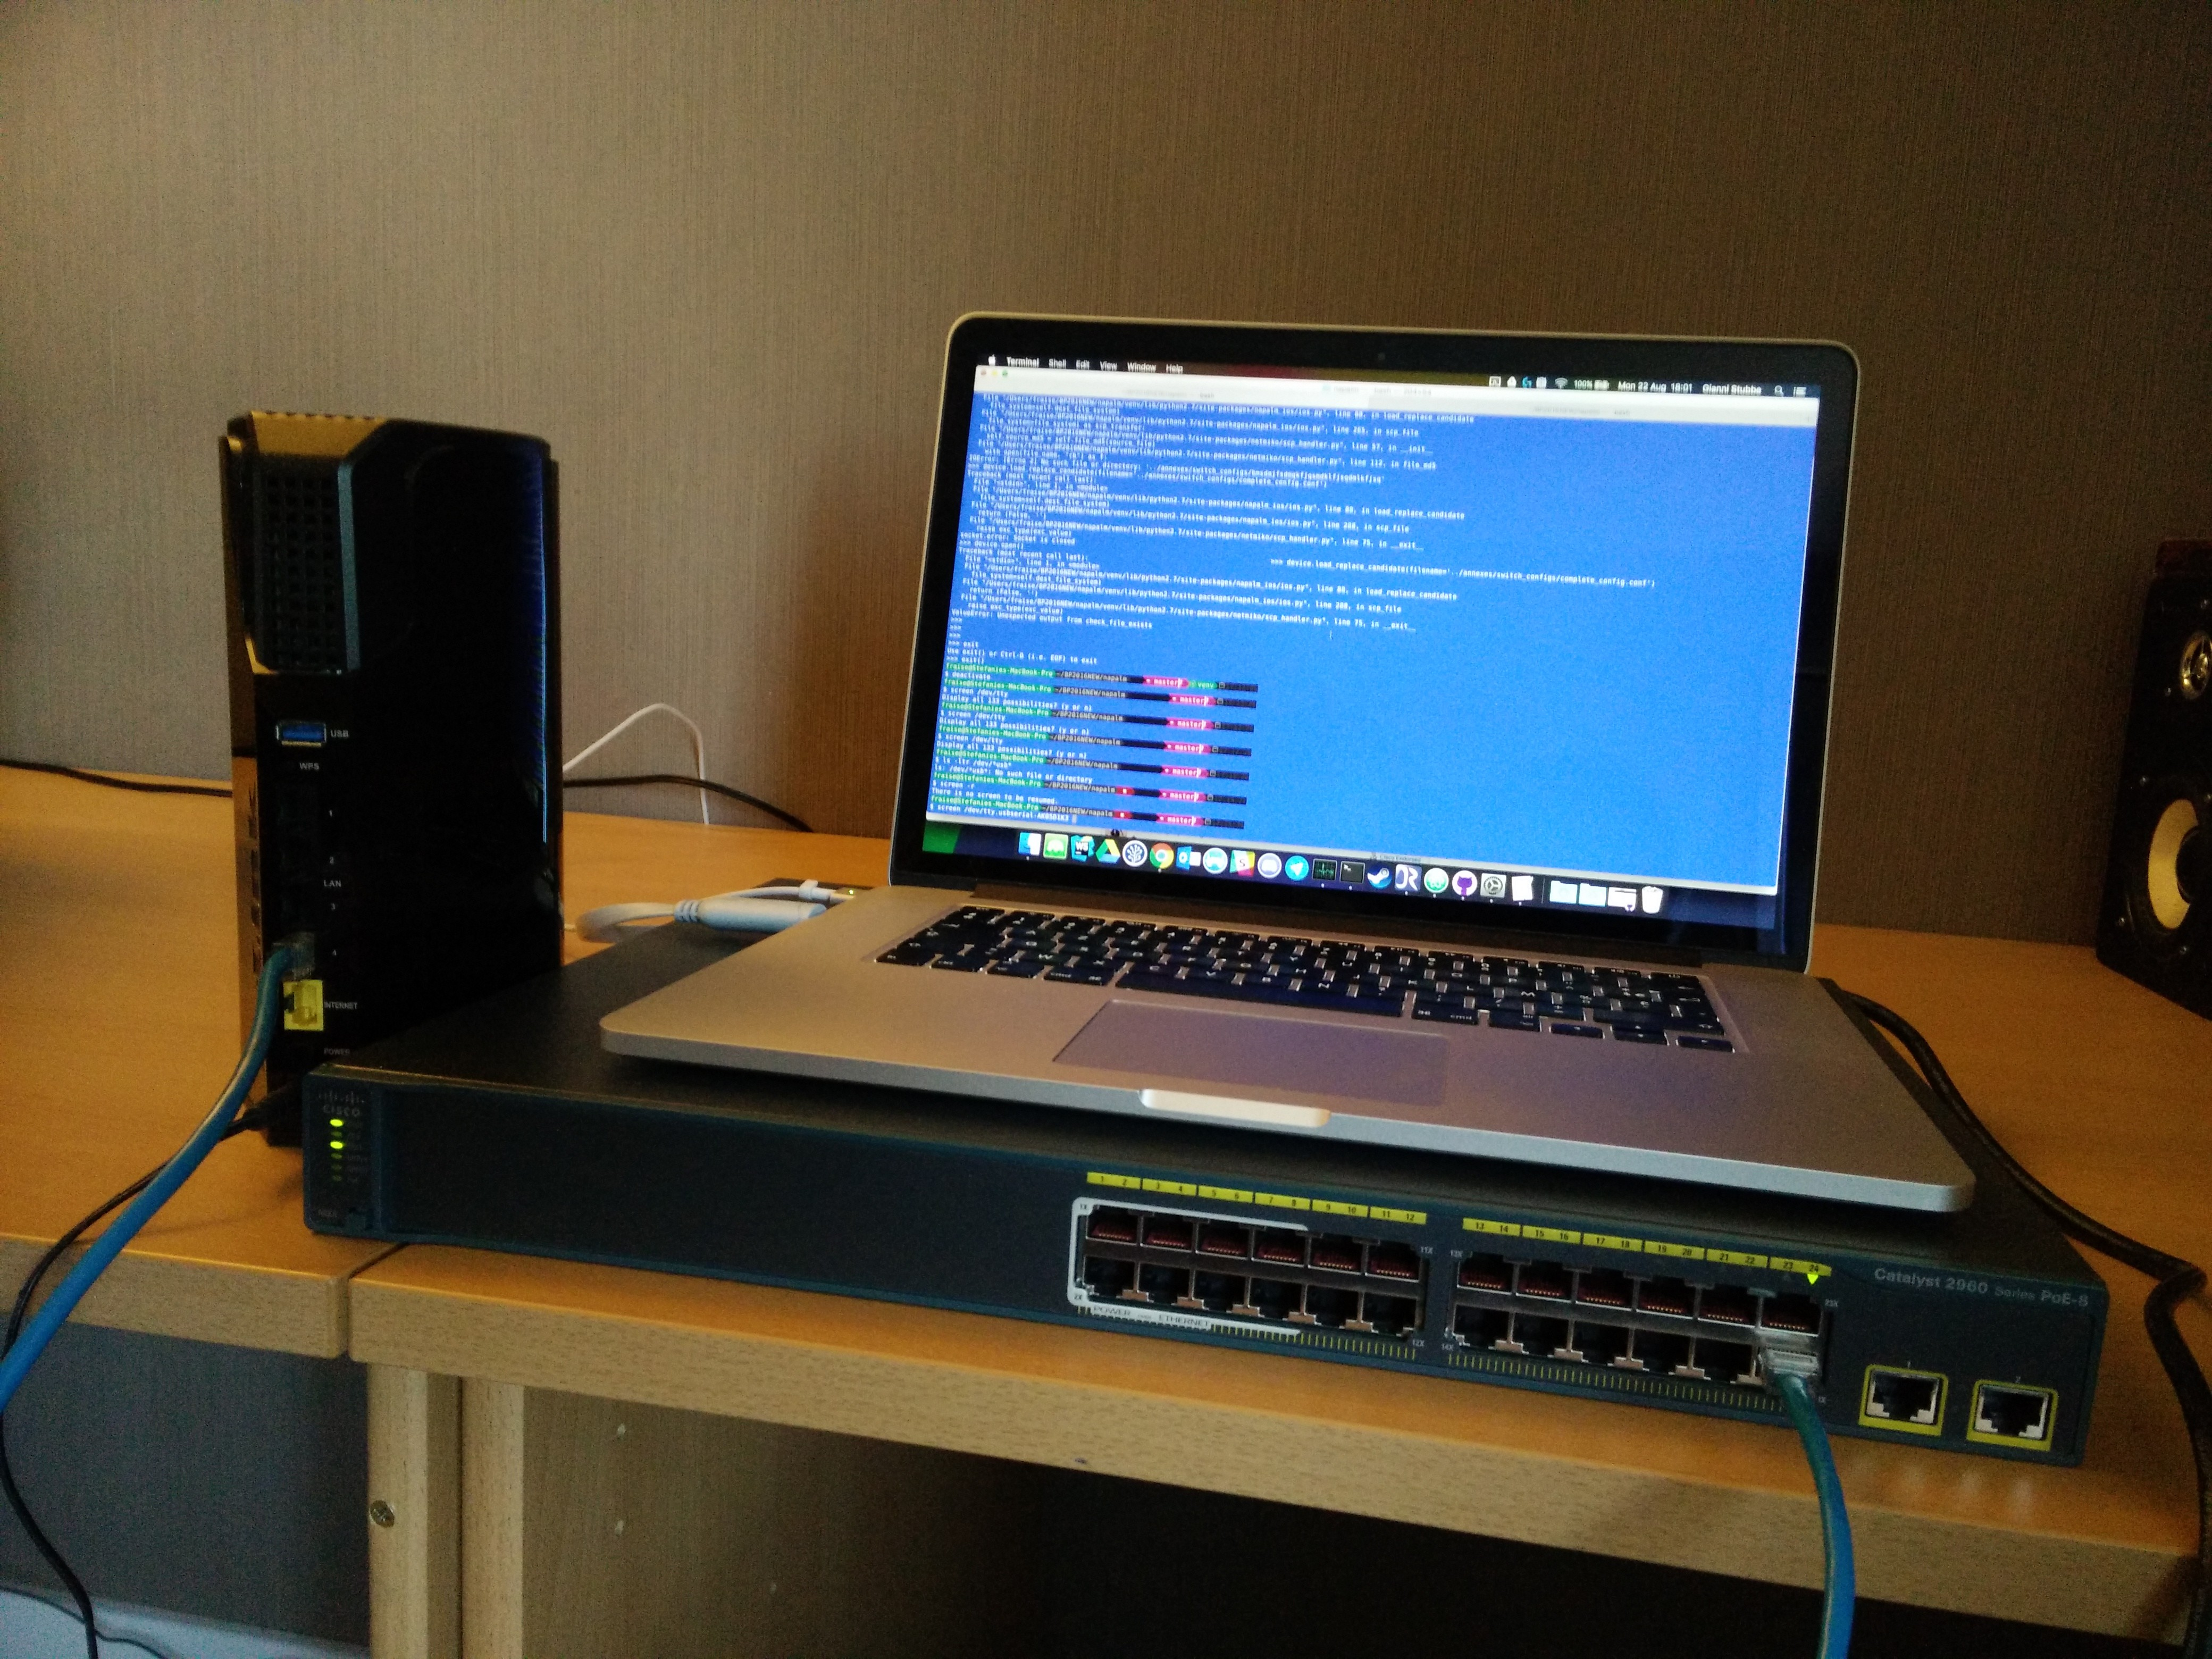
\includegraphics[width=15cm]{../img/setup}
\caption{Links op de afbeelding de router met ip adres: 172.17.1.1 deze is aangesloten op de switch poort fa0/24. Deze behoort tot vlan1 die het ip adres 172.17.1.2 heeft. Daarboven een laptop die via usb console kabel aan de switch verbonden is en via wifi aan de router. Op deze manier was het eenvoudig de switch resetten via console kabel en eenvoudig Ansible uit te voeren over WiFi dan. }
\end{figure}

Na het opstellen van deze testopstelling werd er over gegaan op het configureren van de switch met de basis instellingen die benodigd zijn voor SSH connecties toe te staan.





%%=============================================================================
%% Configuratie
%%=============================================================================

\chapter{Configuratie zonder automatisatie}
\label{ch:configuratie}


Bijlage: Switch Commands.md

Voor de testen zal er gebruik gemaakt worden van een Cisco IOS switch geproduceert in 2006. Deze is een 2960 Series switch en meer bepaald de C2960-24LT. Deze heeft 8 poorten met POE en 2 Gigabit interfaces. 

Deze zal geconfigureerd worden op basis van een een oefening uit de CCNA cursus.

Bijlage: cisco excercise example.pdf\\
Bijlage: -does not exist yet- final configuration


%%=============================================================================
%% Configuratie
%%=============================================================================

\chapter{Automatisatie in combinatie met Ansible}
\label{ch:ansible}
Waar het nu wel allemaal om draait is natuurlijk het automatiseren van alles binnen de Ansible structuur. Er werd een playbook opgemaakt met de basisstructuur en daar werd geleidelijk aan de benodigde configuratie aan toegevoegd.

\section{Configuratie Ansible}
\label{ch:ansibleconfiguratie}
Voor het gebruik van Ansible in combinatie met de 'network-modules' heb je de laatste release nodig van Ansible. Bij het schrijven is dit 2.1.1.0. Deze heeft enkele bug fixes voor netwerk apparatuur. De minimale vereiste voor de ondersteuning van  de netwerkapparatuur is versie 2.1.0.0, dit was de officiële release van de netwerk modules in de core modules. \autocite{ansiblechangelog}
\\

Verder is er een moeilijke keuze geweest qua besturingssysteem om de Ansible rol op uit te voeren. Er werd eerst gekozen om gebruik te maken van een MacBook met de laatste versie 'El Capitan'. Na heel wat zoeken en na het testen van de development release vanaf source bleef er een probleem aanhouden met de 'paramiko' package die nodig is om te kunnen communiceren met netwerkapparaten. Daarna werd er gebruik gemaakt van een laptop waar Ubuntu 16.04 LTS op staat. Ook hier werd de laatste release en development versie op getest. Alles leek te werken maar er bleek een probleem met de ios\_config module. Dus om het toch nog even te testen werd er naar Windows opgestart en werd er gebruik gemaakt van het nieuwe 'Bash on Ubuntu on Windows'. Ook hier werd de laatste release versie getest en de laatste versie die in ontwikkeling is. Ook hier kwam het probleem terug met de ios\_config module.
\\

Verdere configuratie verliep dan verder via de nieuwe implementatie 'Bash on Ubuntu on Windows' (die beschikbaar is geworden met de Windows 10 Anniversary Update) wat verassend genoeg volledig werkte op ieder ander vlak. Hou er wel rekening mee dat deze moet opgestart worden als administrator omdat anders bepaalde netwerkmogelijkheden niet beschikbaar zijn voor bash. Het is een goeie vooruitgang om ook apparaten te kunnen configureren met Ansible vanaf een Windows apparaat. Dit staat natuurlijk los van het onderzoek maar is wel interessant om even op te merken daar het verder onderzoek vanaf een Windows apparaat verliep. 
\\

\begin{figure}[H]
\centering

\includegraphics[width=5cm]{../img/bashonwindows}
\caption{Bash in Windows of via de correcte term 'Bash on Ubuntu on Windows' }
\end{figure}

Verder zal er niet ingegaan worden op vlak van installatie van Ansible. Er wordt verwacht dat de basis van Ansible beschikbaar is op het controlerend apparaat.

\section{Ansible Playbook}
\label{ch:ansibleplaybook}
Bij het schrijven van de playbook voor Ansible werd er zoveel mogelijk gebruik gemaakt van de verschillende mogelijkheden om te tonen wat er momenteel ongeveer al allemaal mogelijk is bij het configureren van netwerksystemen. Verder werden de rollen voor verschillende apparaten opgedeeld in een logische structuur per functie. 
\\

De werkelijke uitvoering van de playbook is er maar gebruik gemaakt van een apparaat namelijk 'switch1'. Er is wel nog ruimte voorzien om dit gemakkelijk uit te breiden naar een tweede apparaat. De configuratie hiervan is wel aangemaakt maar staat in commentaar. De volledige opstelling kan je vinden onderaan in de bijlagen. Verder werd er hier geen gebruik gemaakt van de module ios\_config omdat deze in de huidige staat voor problemen zorgt. Dit is wel de aan te raden manier om configuratie wijzigingen te doen omdat deze zal kijken wat er in de huidige configuratie staat. De ios\_command module die in deze playbook is gebruikt is dus niet de ideale manier maar kan wel werken met variabelen en templating wat je niet hebt bij het gewoon aanmaken van een configuratie.
\\

Om een idee te geven van hoe de ios\_config module precies werkt is er wel een 'common-config' rol toegevoegd die hetzelfde doet als de 'common-command' rol. Dit om aan te tonen hoe het wel correct zou kunnen zijn.

\subsection{Belangrijke Playbook Onderdelen}
\label{ch:ansibleplaybookonderdelen}
Vervolgens zal er wat dieper ingegaan worden op enkele specifieke onderdelen uit de playbook die kenmerkend zijn voor de network-modules.
\\

Een van de belangrijkste onderdelen zijn de login gegevens voor toegang te krijgen tot de switch. Je kan deze afzonderlijk meegeven bij iedere task maar het is eenvoudiger om deze als een host of group variable mee te geven. Dit is mogelijk door de parameter 'provider' die beschikbaar is bij iedere ios module. Deze ondersteund de parameters die onder de module terecht horen in een object, speciaal voor het eenvoudig maken van templating. Verder moet ook de transport parameter meegegeven worden om de correcte connectie te kunnen maken, dit is 'cli' voor deze apparaten.
\\

Verder is er gebruik gemaakt van hashes als variabelen. Dit maakt het heel eenvoudig om commando's die heel hard op elkaar lijken te herhalen. Dit kan bijvoorbeeld het instellen van interfaces zijn of zoals hier bijvoorbeeld het toevoegen van vlans.

\begin{center}
\begin{BVerbatim}
# roles/vlan/tasks/main.yaml
- name: set vlans
  ios_command:
    commands:
      - conf t
      - vlan {{ item.key }}
      - name {{ item.value.name }}
    provider: "{{ cli }}"
  with_dict: "{{ vlans }}"
  
# host_vars/switch1.yaml
vlans:
  99:
    name: management
  10:
    name: faculty-staff
  20:
    name: students
  30:
    name: guest
\end{BVerbatim}
\end{center}

Verder is er ook nog een inventory file gebruikt met geneste groepen. Als hoofdgroepen hebben we namelijk 'routers' en 'switches'. Maar onder switches zit er een subcategorie 'server-switches' en 'client-switches' die het zo mogelijk maakt om heel eenvoudig verschillende configuraties te sturen naar de verschillende groepen switches. Een client heeft bijvoorbeeld geen vlan rol, in de toekomst zouden hier nog andere verschillen kunnen bijkomen.

\subsection{Uitvoeren Playbook}
\label{ch:ansibleplaybookexecution}

Na dat de volledige configuratie aangemaakt was werd deze opnieuw uitgevoerd tegen een switch die terug werd gezet naar de minimale configuratie die nodig is om er van op afstand mee te connecteren via SSH. Nadien werd de configuratie naast elkaar geplaatst om te kijken wat het restultaat was. Onderstaande uitvoer van Ansible toont dat de playbook volledig correct werd uitgevoerd.

\begin{center}
\begin{BVerbatim}

ubuntu@LAPTOP-GIANNI:/mnt/c/Users/Gianni/Documents/GitHub/BP2016NEW/
    ansible$ ansible-playbook ios.yml -i inventory

PLAY [server-switches] ****************************************************

TASK [common-command : set hostname] **************************************
ok: [switch1]

TASK [common-command : disable service 'config'] **************************
ok: [switch1]

TASK [vtp : set vlans] ****************************************************
ok: [switch1]

TASK [trunking : set interfaces 1-5 as trunk ports] ***********************
ok: [switch1]

TASK [trunking : set ip trunk vlan] ***************************************
ok: [switch1]

TASK [vlan : set vlans] ***************************************************
ok: [switch1] => (item={'value': {u'name': u'faculty-staff'}, 'key': 10})
ok: [switch1] => (item={'value': {u'name': u'management'}, 'key': 99})
ok: [switch1] => (item={'value': {u'name': u'students'}, 'key': 20})
ok: [switch1] => (item={'value': {u'name': u'guest'}, 'key': 30})

TASK [vlan : assign interfaces to vlans] **********************************
ok: [switch1] => (item={'value': {u'vlan': 30}, 'key': u'6-10'})
ok: [switch1] => (item={'value': {u'vlan': 10}, 'key': u'11-17'})
ok: [switch1] => (item={'value': {u'vlan': 20}, 'key': u'18-23'})

TASK [vlan : set spanning-tree] *******************************************
ok: [switch1]

TASK [saveconfig : save running-config to startup-config] *****************
ok: [switch1]

PLAY RECAP ****************************************************************
switch1               : ok=9    changed=0    unreachable=0    failed=0

\end{BVerbatim}
\end{center}

Na het uitvoeren van de Ansible rol bleek dan ook dat de configuratie identiek gelijk was aan elkaar. 

\section{Conclusie}
\label{ch:ansibleconclusion}
We kunnen hier uit besluiten dat Ansible op zich correct werkt met netwerkapparatuur. Het biedt extra mogelijkheid tot over het gewoon configureren wat het een heel stuk overzichtelijker maakt en eenvoudiger om een groot netwerkpark te beheren. Het nadeel is wel dat de module ios\_config nog niet werkt. Deze heeft duidelijker weer wat de precieze wijzigingen zijn die toegepast zijn op de configuratie. Eenmaal deze module volledig werkende is lijkt dit een goede optie om het configureren van Cisco IOS apparatuur te automatiseren.

Voor dit aan te kaarten is als de optimale manier van automatisatie voor Cisco apparatuur zal de tegenhanger NAPALM op de test gezet worden.
%%=============================================================================
%% Configuratie
%%=============================================================================

\chapter{Automatisatie in combinatie met NAPALM}
\label{ch:napalm}
Naast Ansible hebben we nog een tweede optie die een heel stuk minder bekend is dan de eerstgenoemde. Dit is NAPALM of ook wel 'Network Automation and Programmability Abstraction Layer with Multivendor support'. Kortgezegd is dit een project geschreven in python om netwerkapparatuur te kunnen aanspreken. Het verschil met ansible zit hem hier in het feit dat je geen tasks gaat definiëren maar dat je een bepaalde configuratie opstelt voor je apparaat en deze daarna test tegenover de huidige configuratie. Voor dat deze naar het apparaat doorgestuurd wordt krijg je een overzicht vergelijkbaar met dat van een git commit waar de wijzigingen zitten in de configuratie. Indien je akkoord bent met de wijzigingen kun je deze 'committen' naar het apparaat of afwijzen om de configuratie te herwerken. 
\\

Een voorbeeld van hoe de wijzigingen worden weergegeven kan je hier onder zien.

\begin{center}
\begin{BVerbatim}
+ hostname pyeos-unittest-changed
- hostname pyeos-unittest
router bgp 65000
   vrf test
     + neighbor 1.1.1.2 maximum-routes 12000
     + neighbor 1.1.1.2 remote-as 1
     - neighbor 1.1.1.1 remote-as 1
     - neighbor 1.1.1.1 maximum-routes 12000
   vrf test2
     + neighbor 2.2.2.3 remote-as 2
     + neighbor 2.2.2.3 maximum-routes 12000
     - neighbor 2.2.2.2 remote-as 2
     - neighbor 2.2.2.2 maximum-routes 12000
interface Ethernet2
+ description ble
- description bla
\end{BVerbatim}
\end{center}

Hoewel dit enkele mogelijkheden biedt die een terminal niet heeft, mist het in vergelijking met Ansible wel nog andere punten die ook een meerwaarde zouden bieden. Een van de grootste voordelen blijft wel het op voorhand zien van de wijzigingen die zullen gebeuren aan je apparaat. Hierdoor is iets over het hoofd zien iets dat minder vaak zal voorkomen. Moest er dan toch nog een foutje in geslopen zijn kan je nog je wijzigingen ongedaan maken met de rollback functionaliteit.

\section{Installatie NAPALM}
\label{ch:napalminstallation}
De installatie van NAPALM is vrij eenvoudig in het eerste opzicht. Als eerste voorwaarde wordt er verwacht van het hostsysteem om Python geïnstalleerd te hebben. 

Eerst en vooral wordt er een virtualenv ingesteld om alles in te runnen, dit zorgt ervoor dat alle dependencies correct zijn specifiek voor deze package en dat de permissies correct zijn. http://docs.python-guide.org/en/latest/dev/virtualenvs/

\begin{center}
\begin{BVerbatim}
$ sudo pip install virtualenv
$ virtualenv venv
$ source venv/bin/activate
\end{BVerbatim}
\end{center}

Daarna wordt NAPALM geïnstalleerd binnen deze virtuele environment via het pip commando.
\begin{center}
\begin{BVerbatim}
(venv)$ pip install napalm
\end{BVerbatim}
\end{center}

\section{Configuratie NAPALM}
\label{ch:napalmconfiguration}

Eenmaal de installatie correct doorlopen is kunnen we aan de slag met de bibliotheek. Hiervoor werden de eerste stappen gevolgd die beschreven staan in de documentatie van NAPALM. Dit beschrijft het uitvoeren van de commando's via de Python shell. Het is natuurlijk ook mogelijk om dit in een python script om te zetten om dit te vereenvoudigen. 
%https://napalm.readthedocs.io/en/latest/tutorials/first_steps_config.html#connecting-to-the-device

\begin{center}
\begin{BVerbatim}
(venv)$ python
>>> from napalm import get_network_driver
>>> driver = get_network_driver('ios')
>>> device = driver('172.17.1.2', 'switchadmin', 'admin')
>>> device.open()
ValueError: An error occurred in dynamically determining
    remote file system: dir Translating "dir"
% Unknown command or computer name, or unable to find computer address
\end{BVerbatim}
\end{center}

Dit is echter waar het misloopt. Bij het proberen connecteren met een Cisco IOS apparaat krijg je de bovenstaande error.
Hoewel je zou denken dat het ip adres dan fout zou zijn geeft dit een andere error terug die weergegen wordt in volgende statement. Hier werd een willekeurig ip adres ingegeven om aan te tonen dat er verschil is met het bovenstaande.

\begin{center}
\begin{BVerbatim}
>>> device = driver('213.213.1.1', 'randomuser', 'randompassword')
>>> device.open()
netmiko.ssh_exception.NetMikoTimeoutException: Connection to 
    device timed-out: cisco_ios 213.213.1.1:22
\end{BVerbatim}
\end{center}

Na wat zoeken op het internet blijkt dat dit een bug is bij de NAPALM bibliotheek. Het deze probeert het 'dir' commando uit te voeren wanneer deze connecteert met het apparaat om te kijken waar de huidige configuratie zich bevindt. Het Cisco apparaat moet daarvoor in de enable mode aanwezig zijn maar het 'enable' commando wordt niet uitgevoerd, noch wordt er ondersteuning geboden voor een enable password. In dezelfde Github issue staat wel uitgelegd hoe we hier omheen kunnen werken. We geven bij het aanmaken van het apparaat een optionele parameter mee die aangeeft waar de directory zich bevindt.

%https://github.com/napalm-automation/napalm-ios/issues/14

%https://napalm.readthedocs.io/en/latest/support/index.html#optional-arguments

\begin{center}
\begin{BVerbatim}
>>> optional_args = {'dest_file_system': 'flash:'}
>>> device = driver('172.17.1.2', 'switchadmin', 
    'cisco', optional_args=optional_args)
>>> device.open()
>>>
\end{BVerbatim}
\end{center}

Nu wordt er met het commando 'load\_replace\_candidate' een configuratie vergeleken met de huidige running config.
Ook hier loopt het jammer genoeg mis. 

\begin{center}
\begin{BVerbatim}
>>> device.load_replace_candidate
    (filename='../annexes/switch_config/complete_config')
ValueError: Unexpected output from check_file_exists
\end{BVerbatim}
\end{center}

Hier keek ik of het niet zou kunnen dat mijn directory structuur niet zou kloppen door en willekeurige bestandsnaam in te geven. Dit bleek een andere error te geven en dus heeft het bovenstaande daar niet mee te maken.

\begin{center}
\begin{BVerbatim}
>>> device.load_replace_candidate
    (filename='../annexes/switch_config/unexisting_config')
IOError: [Errno 2] No such file or directory: 
     '../annexes/switch_config/unexisting_config'
\end{BVerbatim}
\end{center}

Dit heeft wederom te maken met de enable functionaliteit die niet aanwezig in in de package. Dit betekend dat momenteel deze bibliotheek niet gebruikt kan worden in combinatie met Cisco IOS apparatuur en het dus voor dagelijks gebruik ook afgeschreven is. Gelukkig is de development wel nog vrij actief dus kan het goed zijn dat deze binnenkort er toch nog de mogelijkheid komt om dit te gebruiken met de IOS apparaten.

\section{NAPALM Ansible Module}
\label{ch:napalmansible}
Naast de gewone python implementatie heeft NAPALM ook een Ansible module die je kan gebruiken in je project. Deze moet je dan toevoegen in je library folder waarna je van de module gebruik kan maken. Hiervoor moet de NAPALM python module wel voor geïnstalleerd zijn op je hostcomputer. 
\\

Wat een toffe combinatie lijkt is dit combineren met de eerder besproken Ansible network modules. Zo zou je eerst het apparaat kunnen configureren met de ios\_command of ios\_config module. Eenmaal deze alles geconfigureerd heeft op het netwerkaparaat kan je nadien nogmaals de volledig gewenste configuratie met NAPALM doorsturen naar het apparaat. Zo kan je kijken of er verschillen zijn tussen wat je device nu draait en wat je zou verwachten. Voor productie lijkt dit dan ook een mooie extra omdat je nog veel duidelijker een beeld terugkrijgt als er iets niet zou kloppen.
\\

Een voorbeeld van het gebruik van de Ansible module zou er er als volgt kunnen uitzien. Dit uit de Github Documentatie van \cite{githubnabalmansible}. https://github.com/napalm-automation/napalm-ansible

\begin{center}
\begin{BVerbatim}
- name: assemble configuration
  assemble:
    src=../compiled/{{ inventory_hostname }}/
    dest=../compiled/{{ inventory_hostname }}/running.conf

 - name: install napalm config
   napalm_install_config:
    hostname={{ inventory_hostname }}
    username={{ user }}
    dev_os={{ os }}
    password={{ passwd }}
    config_file=../compiled/{{ inventory_hostname }}/running.conf
    commit_changes={{ commit_changes }}
    get_diffs=True
    diff_file=../compiled/{{ inventory_hostname }}/diff
\end{BVerbatim}
\end{center}


\section{Conclusie}
\label{ch:napalconclusie}
NAPALM kan een grote vooruitgang zijn op de huidige werking bij het configureren van een netwerkapparaat. Hoewel er nog vaak aan gewerkt lijkt te worden mist er toch nog de volledige ondersteuning voor Cisco IOS apparaten. Daarom is dit voor het gebruik in combinatie met die apparatuur nog niet mogelijk om dit te gebruiken.
\\

Verder kunnen we wel besluiten dat de beloofde mogelijkheden een goede manier zijn om configuratiewijzigingen overzichtelijk te kunnen weergeven. Dit maakt het wijzigen van configuraties veiliger om te doen en beter maar vooral automatisch gedocumenteerd.
%%=============================================================================
%% Conclusie
%%=============================================================================

\chapter{Conclusie}
\label{ch:conclusie}

%% TODO: Trek een duidelijke conclusie, in de vorm van een antwoord op de
%% onderzoeksvra(a)g(en). Wat was jouw bijdrage aan het onderzoeksdomein en
%% hoe biedt dit meerwaarde aan het vakgebied/doelgroep? Reflecteer kritisch
%% over het resultaat. Had je deze uitkomst verwacht? Zijn er zaken die nog
%% niet duidelijk zijn? Heeft het ondezoek geleid tot nieuwe vragen die
%% uitnodigen tot verder onderzoek?

\lipsum[76-80]



%%---------- Back matter ------------------------------------------------------
%%=============================================================================
%% Configuratie
%%=============================================================================


\chapter*{Bijlagen}
\label{ch:bijlagen}
\addcontentsline{toc}{chapter}{\textcolor{maincolor}Bijlagen}

\setcounter{section}{0}
\renewcommand\thesection{\Alph{section}}

\section{Ansible Playbook}
\label{ch:ansibleplaybookannex}

\begin{BVerbatim}
.
|-- group_vars
|   `-- switches.yaml
|-- host_vars
|   |-- switch1.yaml
|   `-- switch2.yaml
|-- roles
|   |-- common-command
|   |   `-- tasks
|   |       `-- main.yaml
|   |-- common-config
|   |   `-- tasks
|   |       `-- main.yaml
|   |-- saveconfig
|   |   `-- tasks
|   |       `-- main.yaml
|   |-- trunking
|   |   `-- tasks
|   |       `-- main.yaml
|   |-- vlan
|   |   `-- tasks
|   |       `-- main.yaml
|   `-- vtp
|       `-- tasks
|           `-- main.yaml
|-- inventory
`-- ios.yaml
\end{BVerbatim}

\begin{Verbatim}[frame=topline, framesep=4mm, label=\fbox{group\_vars/switches.yaml}]
cli:
  host: "{{ management_ip }}"
  username: "switchadmin"
  password: "cisco"
  authorize: yes
  auth_pass: "class"
  transport: cli
\end{Verbatim}

\begin{Verbatim}[frame=topline, framesep=4mm, label=\fbox{host\_vars/switch1.yaml}]
management_ip: 172.17.1.2

vlan99_ip: "172.17.99.11 255.255.255.0"

vlans:
  99:
    name: management
  10:
    name: faculty-staff
  20:
    name: students
  30:
    name: guest

interfaces:
  6-10:
    vlan: 30
  11-17:
    vlan: 10
  18-23:
    vlan: 20

vtp: server
\end{Verbatim}
\begin{Verbatim}[frame=topline, framesep=4mm, label=\fbox{host\_vars/switch2.yaml}]
management_ip: 172.17.1.3

vlan99_ip: "172.17.99.12 255.255.255.0"

vtp: client
\end{Verbatim}
\begin{Verbatim}[frame=topline, framesep=4mm, label=\fbox{roles/common-command/tasks/main.yaml}]
- name: set hostname
  ios_command:
    commands:
      - conf t
      - hostname "{{ inventory_hostname }}"
    provider: "{{ cli }}"


- name: disable service 'config'
  ios_command:
    commands:
      - conf t
      - no service config
    provider: "{{ cli }}"
\end{Verbatim}
\begin{Verbatim}[frame=topline, framesep=4mm, label=\fbox{roles/common-config/tasks/main.yaml}]
- name: set hostname
  ios_config:
    lines:
      - ['hostname {{inventory_hostname}}']
    provider: "{{ cli }}"

- name: disable service 'config'
  ios_config:
    lines:
      - ['no service config']
    provider: "{{ cli }}"
\end{Verbatim}
\begin{Verbatim}[frame=topline, framesep=4mm, label=\fbox{roles/saveconfig/tasks/main.yaml}]    
- name: save running-config to startup-config
  ios_command:
    commands:
      - write memory
    provider: "{{ cli }}"
\end{Verbatim}
\begin{Verbatim}[frame=topline, framesep=4mm, label=\fbox{roles/trunking/tasks/main.yaml}]       
- name: set interfaces 1-5 as trunk ports
  ios_command:
    commands:
      - conf t
      - int range fa0/1-5
      - switchport mode trunk
      - switchport trunk native vlan 99
      - no shutdown
    provider: "{{ cli }}"

- name: set ip trunk vlan
  ios_command:
    commands:
      - conf t
      - int vlan99
      - ip address {{ vlan99_ip }}
    provider: "{{ cli }}"
\end{Verbatim}
\begin{Verbatim}[frame=topline, framesep=4mm, label=\fbox{roles/vlan/tasks/main.yaml}]
- name: set vlans
  ios_command:
    commands:
      - conf t
      - vlan {{ item.key }}
      - name {{ item.value.name }}
    provider: "{{ cli }}"
  with_dict: "{{ vlans }}"

- name: assign interfaces to vlans
  ios_command:
    commands:
      - conf t
      - int range fa0/{{ item.key }}
      - switchport access vlan {{ item.value.vlan }}
    provider: "{{ cli }}"
  with_dict: "{{ interfaces }}"

- name: set spanning-tree
  ios_command:
    commands:
      - conf t
      - spanning-tree vlan 99 priority 4096
    provider: "{{ cli }}"
\end{Verbatim}
\begin{Verbatim}[frame=topline, framesep=4mm, label=\fbox{roles/vtp/tasks/main.yaml}]
- name: set vlans
  ios_command:
    commands:
      - conf t
      - vtp mode {{ vtp }}
      - vtp domain Lab5
      - vtp password cisco
    provider: "{{ cli }}"

\end{Verbatim}
\begin{Verbatim}[frame=topline, framesep=4mm, label=\fbox{./inventory}]
[routers]
router1

[server-switches]
switch1

[client-switches]
switch2

[switches:children]
server-switches
client-switches
\end{Verbatim}
\begin{Verbatim}[frame=topline, framesep=4mm, label=\fbox{group\_vars/switches.yaml}]
- hosts: server-switches
  gather_facts: no
  connection: local

  vars:
    limit_to: "*"

  roles:
    - common-command
#   - common-config
    - vtp
    - trunking
    - vlan
    - saveconfig

#- hosts: client-switches
#  gather_facts: no
#  connection: local
#
#  vars:
#    limit_to: "*"
#
#  roles:
#    - common-command
##  - common-config
#    - vtp
#    - trunking
#    - saveconfig

\end{Verbatim}

\section{Switch Configuration Files }
\label{ch:switchconfigsannexes}

\begin{Verbatim}[frame=topline, framesep=4mm, label=\fbox{Switch Commands}]

# all switches (except for a unique ip address)

en
conf t
ip default-gateway 172.17.1.1
int vlan1
ip address 172.17.1.2 255.255.255.0
no shut
exit
hostname switchname
ip domain-name website.be
crypto key generate rsa
2048
username switchadmin password cisco
enable secret class
no ip domain-lookup
line console 0
logging synchronous
login local
line vty 0 4
transport input ssh
login local
password cisco
exit
service password-encryption
end
write memory
reload

.

# Switch 1
en
class
conf t
vtp mode server
vtp domain Lab5
vtp password cisco
int range fa0/1-5
switchport mode trunk
switchport trunk native vlan 99
no shutdown
exit
vlan 99
name management
vlan 10
name faculty-staff
vlan 20
name students
vlan 30
name guest
exit
int vlan99
ip address 172.17.99.11 255.255.255.0
exit
int range fa0/6-10
switchport access vlan 30
int range fa0/11-17
switchport access vlan 10
int range fa0/18-23
switchport access vlan 20
exit
spanning-tree vlan 99 priority 4096
end
write memory
reload

.

# Optional Switch 2

vtp mode client
vtp domain Lab5
vtp password cisco
end
int range fa0/1-5
switchport mode trunk
switchport trunk native vlan 99
no shut
int vlan99
ip address 172.17.99.12 255.255.255.0
end
write memory

\end{Verbatim}
\begin{Verbatim}[frame=topline, framesep=4mm, label=\fbox{Initial Switchconfig}]

Current configuration : 1274 bytes
!
version 12.2
no service pad
service timestamps debug datetime msec
service timestamps log datetime msec
no service password-encryption
!
hostname Switch
!
boot-start-marker
boot-end-marker
!
!
no aaa new-model
system mtu routing 1500
ip subnet-zero
!
!
!
!
!
!
!
!
!
spanning-tree mode pvst
spanning-tree extend system-id
!
vlan internal allocation policy ascending
!
!
!
interface FastEthernet0/1
!
interface FastEthernet0/2
!
interface FastEthernet0/3
!
interface FastEthernet0/4
!
interface FastEthernet0/5
!
interface FastEthernet0/6
!
interface FastEthernet0/7
!
interface FastEthernet0/8
!
interface FastEthernet0/9
!
interface FastEthernet0/10
!
interface FastEthernet0/11
!
interface FastEthernet0/12
!
interface FastEthernet0/13
!
interface FastEthernet0/14
!
interface FastEthernet0/15
!
interface FastEthernet0/16
!
interface FastEthernet0/17
!
interface FastEthernet0/18
!
interface FastEthernet0/19
!
interface FastEthernet0/20
!
interface FastEthernet0/21
!
interface FastEthernet0/22
!
interface FastEthernet0/23
!
interface FastEthernet0/24
!
interface GigabitEthernet0/1
!
interface GigabitEthernet0/2
!
interface Vlan1
 no ip address
 no ip route-cache
 shutdown
!
ip http server
ip http secure-server
!
control-plane
!
!
line con 0
line vty 5 15
!
end

VLAN Name                             Status    Ports
---- -------------------------------- --------- -------------------------------
1    default                          active    Fa0/1, Fa0/2, Fa0/3, Fa0/4
                                                Fa0/5, Fa0/6, Fa0/7, Fa0/8
                                                Fa0/9, Fa0/10, Fa0/11, Fa0/12
                                                Fa0/13, Fa0/14, Fa0/15, Fa0/16
                                                Fa0/17, Fa0/18, Fa0/19, Fa0/20
                                                Fa0/21, Fa0/22, Fa0/23, Fa0/24
                                                Gi0/1, Gi0/2
1002 fddi-default                     act/unsup
1003 token-ring-default               act/unsup
1004 fddinet-default                  act/unsup
1005 trnet-default                    act/unsup
\end{Verbatim}
\begin{Verbatim}[frame=topline, framesep=4mm, label=\fbox{Minimal Switchconfig}]

Current configuration : 3226 bytes
!
version 12.2
no service pad
service timestamps debug datetime msec
service timestamps log datetime msec
service password-encryption
!
hostname Switch
!
boot-start-marker
boot-end-marker
!
enable secret 5 $1$ad1E$eENpnWdsRwvYDTMRFlbDU1
!
username switchadmin password 7 070C285F4D06
no aaa new-model
system mtu routing 1500
ip subnet-zero
!
no ip domain-lookup
ip domain-name website.be
!
!
crypto pki trustpoint TP-self-signed-3395035520
 enrollment selfsigned
 subject-name cn=IOS-Self-Signed-Certificate-3395035520
 revocation-check none
 rsakeypair TP-self-signed-3395035520
!
!
crypto pki certificate chain TP-self-signed-3395035520
 certificate self-signed 01
  30820249 308201B2 A0030201 02020101 300D0609 2A864886 F70D0101 04050030
  31312F30 2D060355 04031326 494F532D 53656C66 2D536967 6E65642D 43657274
  69666963 6174652D 33333935 30333535 3230301E 170D3933 30333031 30303030
  35385A17 0D323030 31303130 30303030 305A3031 312F302D 06035504 03132649
  4F532D53 656C662D 5369676E 65642D43 65727469 66696361 74652D33 33393530
  33353532 3030819F 300D0609 2A864886 F70D0101 01050003 818D0030 81890281
  8100A673 DFD43E3D 3BE774FD 0CB6712E A10DE672 23FEAB25 17958BA9 ED53EF31
  16E89D4B D12CC2BF C3F01FA9 F59BB01D C357FF77 326CA8B6 EDE96337 8F9FE592
  A130BE8A 855DFE7F B6244C18 599619CC 332DCDAB 47820375 C3178B35 716936BA
  66C276C6 E64E93C3 0742C86B 5392508F 479A4BEF 77D02D10 2E651B8B 890B5AAB
  4C6F0203 010001A3 71306F30 0F060355 1D130101 FF040530 030101FF 301C0603
  551D1104 15301382 11537769 7463682E 77656273 6974652E 6265301F 0603551D
  23041830 16801477 D48AFA9A FABC2C8F ADA95327 05318386 80905C30 1D060355
  1D0E0416 041477D4 8AFA9AFA BC2C8FAD A9532705 31838680 905C300D 06092A86
  4886F70D 01010405 00038181 004087FF 7549472F 7A4F0F86 5679CCF6 E7181F92
  3ADD4015 4E9FA2E7 B01FDF33 A21201B7 9EFBBA7A 84517C3D 8344650C 5059EB07
  C3A063FD 24A56FDC BEC1ADA8 0FD8C3DE 1F06EBB2 2F102D9E 16191DFB D56291D2
  072E7607 FF83C621 1281B7D0 68B8F6DC ED15CE01 7ED31165 ACE71D37 AA5E2538
  476F348E 65D8C7CE EF0F32A6 F3
  quit
!
!
!
!
!
spanning-tree mode pvst
spanning-tree extend system-id
!
vlan internal allocation policy ascending
!
!
!
interface FastEthernet0/1
!
interface FastEthernet0/2
!
interface FastEthernet0/3
!
interface FastEthernet0/4
!
interface FastEthernet0/5
!
interface FastEthernet0/6
!
interface FastEthernet0/7
!
interface FastEthernet0/8
!
interface FastEthernet0/9
!
interface FastEthernet0/10
!
interface FastEthernet0/11
!
interface FastEthernet0/12
!
interface FastEthernet0/13
!
interface FastEthernet0/14
!
interface FastEthernet0/15
!
interface FastEthernet0/16
!
interface FastEthernet0/17
!
interface FastEthernet0/18
!
interface FastEthernet0/19
!
interface FastEthernet0/20
!
interface FastEthernet0/21
!
interface FastEthernet0/22
!
interface FastEthernet0/23
!
interface FastEthernet0/24
!
interface GigabitEthernet0/1
!
interface GigabitEthernet0/2
!
interface Vlan1
 ip address 172.17.1.2 255.255.255.0
 no ip route-cache
!
ip default-gateway 172.17.1.1
ip http server
ip http secure-server
!
control-plane
!
!
line con 0
 logging synchronous
 login local
line vty 0 4
 password 7 14141B180F0B
 login local
 transport input ssh
line vty 5 15
 login
 !
end

VLAN Name                             Status    Ports
---- -------------------------------- --------- -------------------------------
1    default                          active    Fa0/1, Fa0/2, Fa0/3, Fa0/4
                                                Fa0/5, Fa0/6, Fa0/7, Fa0/8
                                                Fa0/9, Fa0/10, Fa0/11, Fa0/12
                                                Fa0/13, Fa0/14, Fa0/15, Fa0/16
                                                Fa0/17, Fa0/18, Fa0/19, Fa0/20
                                                Fa0/21, Fa0/22, Fa0/23, Fa0/24
                                                Gi0/1, Gi0/2
1002 fddi-default                     act/unsup
1003 token-ring-default               act/unsup
1004 fddinet-default                  act/unsup
1005 trnet-default                    act/unsup 

\end{Verbatim}
\begin{Verbatim}[frame=topline, framesep=4mm, label=\fbox{Complete Switchconfig}]

Current configuration : 4110 bytes
!
version 12.2
no service pad
service timestamps debug datetime msec
service timestamps log datetime msec
service password-encryption
!
hostname switch1
!
boot-start-marker
boot-end-marker
!
enable secret 5 $1$ad1E$eENpnWdsRwvYDTMRFlbDU1
!
username switchadmin password 7 070C285F4D06
no aaa new-model
system mtu routing 1500
ip subnet-zero
!
no ip domain-lookup
ip domain-name website.be
!
!
crypto pki trustpoint TP-self-signed-3395035520
 enrollment selfsigned
 subject-name cn=IOS-Self-Signed-Certificate-3395035520
 revocation-check none
 rsakeypair TP-self-signed-3395035520
!
!
crypto pki certificate chain TP-self-signed-3395035520
 certificate self-signed 01
  3082024A 308201B3 A0030201 02020101 300D0609 2A864886 F70D0101 04050030
  31312F30 2D060355 04031326 494F532D 53656C66 2D536967 6E65642D 43657274
  69666963 6174652D 33333935 30333535 3230301E 170D3933 30333031 30303030
  35355A17 0D323030 31303130 30303030 305A3031 312F302D 06035504 03132649
  4F532D53 656C662D 5369676E 65642D43 65727469 66696361 74652D33 33393530
  33353532 3030819F 300D0609 2A864886 F70D0101 01050003 818D0030 81890281
  8100A673 DFD43E3D 3BE774FD 0CB6712E A10DE672 23FEAB25 17958BA9 ED53EF31
  16E89D4B D12CC2BF C3F01FA9 F59BB01D C357FF77 326CA8B6 EDE96337 8F9FE592
  A130BE8A 855DFE7F B6244C18 599619CC 332DCDAB 47820375 C3178B35 716936BA
  66C276C6 E64E93C3 0742C86B 5392508F 479A4BEF 77D02D10 2E651B8B 890B5AAB
  4C6F0203 010001A3 72307030 0F060355 1D130101 FF040530 030101FF 301D0603
  551D1104 16301482 12737769 74636831 2E776562 73697465 2E626530 1F060355
  1D230418 30168014 77D48AFA 9AFABC2C 8FADA953 27053183 8680905C 301D0603
  551D0E04 16041477 D48AFA9A FABC2C8F ADA95327 05318386 80905C30 0D06092A
  864886F7 0D010104 05000381 81006AA2 B75C7693 7562D9CC DC1F2EA7 1C686C77
  F8536E96 FB7EF881 F8CEB1C7 1E2BDFDD 4248806D 87424281 24B4940C 8FF74A21
  059C9F53 AF3C49C8 C2DF7262 FC20015C 31AA9A8A B9B850CA 40700B80 323E1CCE
  D1397329 14FB561C AD0445DC DD666155 4AEC3C75 6B48B2E6 85ACA015 C40D6F26
  7455E576 FDC95466 CFAD97D9 F5C2
  quit
!
!
!
!
!
!
spanning-tree mode pvst
spanning-tree extend system-id
spanning-tree vlan 99 priority 4096
!
vlan internal allocation policy ascending
!
!
!
interface FastEthernet0/1
 switchport trunk native vlan 99
 switchport mode trunk
!
interface FastEthernet0/2
 switchport trunk native vlan 99
 switchport mode trunk
!
interface FastEthernet0/3
 switchport trunk native vlan 99
 switchport mode trunk
!
interface FastEthernet0/4
 switchport trunk native vlan 99
 switchport mode trunk
!
interface FastEthernet0/5
 switchport trunk native vlan 99
 switchport mode trunk
!
interface FastEthernet0/6
switchport access vlan 30
!
interface FastEthernet0/7
switchport access vlan 30
!
interface FastEthernet0/8
switchport access vlan 30
!
interface FastEthernet0/9
switchport access vlan 30
!
interface FastEthernet0/10
switchport access vlan 30
!
interface FastEthernet0/11
switchport access vlan 10
!
interface FastEthernet0/12
switchport access vlan 10
!
interface FastEthernet0/13
switchport access vlan 10
!
interface FastEthernet0/14
switchport access vlan 10
!
interface FastEthernet0/15
switchport access vlan 10
!
interface FastEthernet0/16
switchport access vlan 10
!
interface FastEthernet0/17
switchport access vlan 10
!
interface FastEthernet0/18
switchport access vlan 20
!
interface FastEthernet0/19
switchport access vlan 20
!
interface FastEthernet0/20
switchport access vlan 20
!
interface FastEthernet0/21
switchport access vlan 20
!
interface FastEthernet0/22
switchport access vlan 20
!
interface FastEthernet0/23
switchport access vlan 20
!
interface FastEthernet0/24
!
interface GigabitEthernet0/1
!
interface GigabitEthernet0/2
!
interface Vlan1
 ip address 172.17.1.2 255.255.255.0
 no ip route-cache
!
interface Vlan99
 ip address 172.17.99.11 255.255.255.0
 no ip route-cache
!
ip default-gateway 172.17.1.1
ip http server
ip http secure-server
!
control-plane
!
!
line con 0
 logging synchronous
 login local
line vty 0 4
 password 7 14141B180F0B
 login local
 transport input ssh
line vty 5 15
 login
!
end


VLAN Name                             Status    Ports
---- -------------------------------- --------- -------------------------------
1    default                          active    Fa0/1, Fa0/2, Fa0/3, Fa0/4
                                                Fa0/5, Fa0/24, Gi0/1, Gi0/2
10   faculty-staff                    active    Fa0/11, Fa0/12, Fa0/13, Fa0/14
                                                Fa0/15, Fa0/16, Fa0/17
20   students                         active    Fa0/18, Fa0/19, Fa0/20, Fa0/21
                                                Fa0/22, Fa0/23
30   guest                            active    Fa0/6, Fa0/7, Fa0/8, Fa0/9
                                                Fa0/10
99   management                       active
1002 fddi-default                     act/unsup
1003 token-ring-default               act/unsup
1004 fddinet-default                  act/unsup
1005 trnet-default                    act/unsup

\end{Verbatim}



\printbibliography
\addcontentsline{toc}{chapter}{\textcolor{maincolor}{\IfLanguageName{dutch}{Bibliografie}{Bibliography}}}


\listoffigures

\end{document}